%% LLT: Turn off some annoying warnings...
\RequirePackage{silence}
\WarningFilter{titlesec}{Non standard sectioning command}
\WarningFilter{scrreprt}{Usage of package}
\WarningFilter{scrreprt}{Activating an ugly workaround}

%This thesis was typeset with \LaTeXe. It uses the \textit{Clean Thesis} style developed by Ricardo Langner. The design of the \textit{Clean Thesis} style is inspired by user guide documents from Apple Inc. The thesis template was adapted by Desmond Grossmann, Stefan Janisch and Paul Beck to implement the editorial guidelines of \textit{Astronomy\A&Astrophysics} and the corporate identity guidelines of the University of Graz for the faculty of natural sciences. 

% **************************************************
% Document Class Definition
% **************************************************

\documentclass[%
	paper=A4,					% paper size --> A4 is default in Germany
	twoside=true,				% onesite or twoside printing
	openright,					% doublepage cleaning ends up right side
	parskip=full,				% spacing value / method for paragraphs
	chapterprefix=true,			% prefix for chapter marks
	11pt,						% font size
	headings=normal,			% size of headings
	bibliography=totoc,			% include bib in toc
	listof=totoc,				% include listof entries in toc
	titlepage=on,				% own page for each title page
	captions=tableabove,		% display table captions above the float env
	draft=false,				% value for draft version
]{scrreprt}%
% **************************************************
% Debug LaTeX Information
% **************************************************
%\listfiles
\usepackage[a-1b]{pdfx}
% **************************************************
% Information and Commands for Reuse
% **************************************************
\usepackage{wrapfig}
\newcommand{\thesisTitle}{De revolutionibus orbium coelestium}
\newcommand{\thesisSubtitle}{Über die Umlaufbahnen der Himmelssphären}
\newcommand{\thesisName}{Nicolaus Copernicus}
\newcommand{\thesisSubject}{Bachelor's / Master's / PhD Thesis}
\newcommand{\thesisDegree}{Bachelor / Master of Science $-$ BSc / MSc}
\newcommand{\thesisDate}{\today}
\newcommand{\thesisVersion}{2.0}


\newcommand{\thesisFirstSupervisor}{Prof.\,Dr. Aristach von Samos}
\newcommand{\thesisSecondSupervisor}{Johannes Kepler, PhD}

\newcommand{\thesisUniversity}{\protect{University of Graz}}
\newcommand{\thesisUniversityDepartment}{Department of Geophysics, Astrophysics and Meteorology}
\newcommand{\thesisUniversityInstitute}{Institute of Physics}
%\newcommand{\thesisUniversityGroup}{Clean Thesis Group (CTG)}
\newcommand{\thesisUniversityCity}{Graz}
\newcommand{\thesisUniversityStreetAddress}{Universitaetsplatz 5}
\newcommand{\thesisUniversityPostalCode}{8020}
%Various shortcuts for journals

\newcommand{\aap}{Astronomy and Astrophysics}
\newcommand{\mnras}{Monthly Notices of the RAS}
\newcommand{\apj}{The Astrophysical Journal}
\newcommand{\Kepler}{\textit{Kepler} }
\newcommand{\apjs}{The Astrophysical Journal Supplement}
\newcommand{\nphysa}{Nuclear Physics A}
\newcommand{\prd}{Physical Review D}

\usepackage{xspace}
\newcommand{\Figure}[1]{Figure\,\ref{#1}\xspace}
\newcommand{\Fig}[1]{Fig.\,\ref{#1}\xspace}
\newcommand{\Equation}[1]{Equation\,\ref{#1}\xspace}
\newcommand{\Eq}[1]{Eq.\,\ref{#1}\xspace}
\newcommand{\Section}[1]{Section\,\ref{#1}\xspace}
\newcommand{\Sec}[1]{Sec.\,\ref{#1}\xspace}

\newcommand{\Table}[1]{Table\,\ref{#1}\xspace}
\newcommand{\Listing}[1]{Listing\,\ref{#1}\xspace}

\usepackage{pdflscape,longtable} % allowing for tables in landscape format and long tables

\usepackage{textgreek} %allow for greek character in text, e.g. \textbeta

\usepackage{setspace, graphicx, hyphenat, fancyhdr, ifthen, everypage, enumitem, setspace}
\usepackage[pdfa]{hyperref}

%\RequirePackage[dvipsnames]{xcolor}
\newcommand{\blu}{\textcolor{blue} }
\newcommand{\red}{\textcolor{red} }
\newcommand{\grn}{\textcolor{green} }
\newcommand{\cya}{\textcolor{cyan} }

\usepackage[normalem]{ulem}
%Loading the normalem package option prevents the redefinition of existing, already loaded definitions. If not loaded, the redefinition of the \emph command through ulem leads to formating problems in the bibilgraphy.


%bold Text in CI-Color
\newcommand{\physbf}[1]{\textbf{\textcolor{ctgreenblue}{#1}}}
%italic Text in CI-Color
\newcommand{\physit}[1]{\textit{\textcolor{ctgreenblue}{#1}}}
%normal Text in CI-Color
\newcommand{\physnormal}[1]{\textcolor{ctgreenblue}{#1}}
\newcommand{\physgray}[1]{\textcolor{ctcolorgray}{#1}}
%horizontal like in CI-Color
\newcommand{\physRules}{{\color{ctcolorgray}{\vspace{-10mm}\rule{\linewidth}{1pt}}}\vspace{-1mm}}
%\newcommand{\physRules}[1]{%\textcolor{black}{\vspace{-9mm}\rule[0.5ex]{\linewidth}{1pt}}}

% iteration Tools: Candidate ---------------------------------------------------
\newcommand{\StudentInitials}{StudentPlaceYourInitialsHere}
\newcommand{\AdviserInitials}{AdviserPlaceYourInitialsHere}

\newcommand{\myRevision}[1]{\textbf{\textcolor{red}{#1}}}
\newcommand{\myComment}[1]{\textit{\textcolor{red}{[\StudentInitials: #1]}}}
\newcommand{\myToDo}[1]{\textit{\textcolor{orange}{[\textsc{ToDo}: #1]}}}


% iteration Tools: Supervisor --------------------------------------------------
\newcommand{\adviserComment}[1]{\textit{\textcolor{blue}{[\AdviserInitials: #1]}}}

%add re
\newcommand{\adviserAddition}[1]{\textbf{\textcolor{blue}{#1}}}

\newcommand{\adviserHighlighted}[1]{\newline\colorbox{yellow}{\parbox{1\textwidth}{#1}}}

\newcommand{\longSentence}[1]
{\newline\colorbox{yellow}{\parbox{1\textwidth}{#1}\textcolor{gray}{~~[\textit{long Sentence}]}}}


\newcommand{\adviserMarkover}[1]{\textit{\textcolor{magenta}{\uwave{#1}}}}
\newcommand{\mo}[1]{\textit{\textcolor{magenta}{\uwave{#1}}}}

\newcommand{\adviserMarkoverComment}[2]{\textit{\textcolor{magenta}{\uwave{#1}}} \textit{\textcolor{blue}{[\AdviserInitials: #2]}}}
\newcommand{\mc}[2]{\textit{\textcolor{magenta}{\uwave{#1}}} \textit{\textcolor{blue}{[\AdviserInitials: #2]}}}

\newcommand{\adviserDelete}[1]{\textit{\textcolor{magenta}{\sout{#1}}}}



%Various useful astronomical commands
\newcommand{\Msun}{\>{\rm M_{\odot}}\xspace}
\newcommand{\Rsun}{\mbox{$R_{\odot}$}\xspace}
\newcommand{\sig}{\mbox{$\sigma_{e}$}\xspace}
\newcommand{\degs} {^\circ}
\newcommand{\numax} {$\nu_{\mathrm{max}}$\xspace}
\newcommand{\dnu} {$\Delta\nu$\xspace}
\newcommand{\muHz}{\,$\mu$Hz\xspace}
\newcommand{\varR}{$\varepsilon_r$\xspace}

% **************************************************
% Load and Configure Packages
% **************************************************
\usepackage{amsmath,amssymb}
\usepackage{pdfpages}
\usepackage[utf8]{inputenc}		% defines file's character encoding
\usepackage[T1]{fontenc}
\usepackage{threeparttable}
\DeclareUnicodeCharacter{00A0}{ }
\usepackage[english]{babel} % babel system, adjust the language of the content
\usepackage{silence}
\WarningFilter{latex}{Text page}
\usepackage{lipsum}

\usepackage[	
    sorting=none,				% clean thesis style
	figuresep=colon,%
	sansserif=false, % true wäre CI standard
	hangfigurecaption=false,%
	hangsection=true,%
	hangsubsection=true,%
	colorize=full,%
	colortheme=bluemagenta,%
% LLT: Use biber if using UTF8 encoding
% 	bibsys=bibtex,%
	bibsys=biber,%
	bibfile=bib-refs,%
	bibstyle=numeric,
    style=numeric,
    backend=biber,%
]{cleanthesis}
%\let\cite\citet
\usepackage[hang]{footmisc}
\setlength{\footnotemargin}{2mm}

%by default Bibtext would use the abbreviation 'u.a.' instead of 'et al.', when set to German. This can be corrected by:
\DefineBibliographyStrings{german}{andothers={et\addabbrvspace al\adddot}}


\hypersetup{					% setup the hyperref-package options
	pdftitle={\thesisTitle},	% 	- title (PDF meta)
	pdfsubject={\thesisSubject},% 	- subject (PDF meta)
	pdfauthor={\thesisName},	% 	- author (PDF meta)
	plainpages=false,			% 	-
	colorlinks=true,			% 	- colorize links?
	citecolor= ctgreenblue,
    linkcolor= ctgreenblue,
    urlcolor= ctgreenblue,
    pdfborder={0 0 0},			% 	-
	breaklinks=true,			% 	- allow line break inside links
	bookmarksnumbered=true,		%
	bookmarksopen=true			%
}

%\usepackage[firstpage]{draftwatermark}\SetWatermarkText{Thesis Template}\SetWatermarkScale{0.5}

% --------------------------
% rename document parts
% --------------------------
\captionsetup{labelfont={sf,bf,color=ctgreenblue},font={color=black}}

%FIGURES
\renewcaptionname{english}{\figurename}{Fig.}
%%%%%%%%%%%%%%%%%%
\usepackage{subcaption}
%%%%%%%%%%%%%%%%%%
%TABLES
\renewcaptionname{english}{\tablename}{Table}
\newcommand{\tablefoot}[1]{\medskip \small \textcolor{ctgreenblue}{\bfseries\sffamily Notes.} #1}
\newcommand{\systemDependencies}[1]{\textcolor{ctgreenblue}{\bfseries\sffamily System Dependencies.} #1}
\newcommand{\monofig}[4]{
    
    \begin{figure}[H]
    \centering
    \includegraphics[#1]{#2}
    \caption{
        #3
    }
    \label{#4}
    \end{figure}
    
}
\newcommand{\polyfig}[6]{
    \begin{figure}[H]
        \centering
        \begin{minipage}[b]{0.45\textwidth}
            \centering
            \includegraphics[width=\textwidth]{#1}
            \caption{#2}
            \label{#3}
        \end{minipage}
        \begin{minipage}[b]{0.45\textwidth}
            \centering
            \includegraphics[width=\textwidth]{#4}
            \caption{#5}
            \label{#6}
        \end{minipage}
    \end{figure}
}
\newcommand{\polyfigacc}[8]{
    \begin{figure}[H]
        \centering
        \begin{minipage}[b]{#1}
            \centering
            \includegraphics[width=\textwidth]{#2}
            \caption{#3}
            \label{#4}
        \end{minipage}
        \begin{minipage}[b]{#5}
            \centering
            \includegraphics[width=\textwidth]{#6}
            \caption{#7}
            \label{#8}
        \end{minipage}
    \end{figure}
}
\newcommand{\trifig}[9]{
    \begin{figure}[H]
        \centering
        \begin{minipage}[b]{0.32\textwidth}
            \centering
            \includegraphics[width=\textwidth]{#1}
            \caption{#2}
            \label{#3}
        \end{minipage}
        \begin{minipage}[b]{0.32\textwidth}
            \centering
            \includegraphics[width=\textwidth]{#4}
            \caption{#5}
            \label{#6}
        \end{minipage}
        \begin{minipage}[b]{0.32\textwidth}
            \centering
            \includegraphics[width=\textwidth]{#7}
            \caption{#8}
            \label{#9}
        \end{minipage}
        \caption{#10}
        \label{#11}
    \end{figure}
}
\newcommand{\trifigcom}[8]{
    \begin{figure}[H]
        \centering
        \begin{subfigure}[b]{0.32\textwidth}
            \centering
            \includegraphics[width=\textwidth]{#1}
            \caption{}
            \label{#2}
        \end{subfigure}
        \begin{subfigure}[b]{0.32\textwidth}
            \centering
            \includegraphics[width=\textwidth]{#3}
            \caption{}
            \label{#4}
        \end{subfigure}
        \begin{subfigure}[b]{0.32\textwidth}
            \centering
            \includegraphics[width=\textwidth]{#5}
            \caption{}
            \label{#6}
        \end{subfigure}
        \caption{#7}
        \label{#8}
    \end{figure}
}
\newcommand{\duofigcom}[6]{
    \begin{figure}[H]
        \centering
        \begin{subfigure}{0.49\textwidth}
            \includegraphics[width=\textwidth]{#1}
            \caption{}
            \label{#2}
        \end{subfigure}
        \begin{subfigure}{0.49\textwidth}
            \includegraphics[width=\textwidth]{#3}
            \caption{}
            \label{#4}
        \end{subfigure}
        \caption{
            #5
            }
        \label{#6}
    \end{figure}
}
\graphicspath{ {./graphics/} }  
\usepackage{float}
%EQUATIONS
%\renewcommand\theequation{{\color{ctgreenblue} \arabic{equation}}}
%\newtagform{physGreen}{\color{RoyalBlue3}(}{)}
%\usetagform{physGreen}


%\patchcmd{\@eqnnum}{\normalcolor}{\color{magenta}}{\typeout{eqnnum patch: OK!}}{\typeout{eqnnum patch: Oh, dear!}}

%LISTING
% printing out color coded python code
%\usepackage{listings,minted}
\usepackage{listings,multicol}
%https://en.wikibooks.org/wiki/LaTeX/Source_Code_Listings
 \definecolor{greencode}{rgb}{0,0.7,0}
 \definecolor{purplecode}{rgb}{0.7,0,0.7}

\lstdefinestyle{spyderstyle}{
	language=Fortran,
    %backgroundcolor=\color{backcolours},   
    frame=Tb,
    basicstyle=\small,
    commentstyle=\color{gray},
    keywordstyle=\color{purplecode},
    numberstyle=\scriptsize\color{gray},
    stringstyle=\color{greencode},               
    numbers=left,     
    classoffset=1,
    keywordstyle=\color{blue},
}
\lstset{style=spyderstyle}

\usepackage[msc,nawi]{tugrazthesis} % TU Graz Title Style
%----------------------------------------------------------


% **************************************************
% Information for TU Titlepage
% **************************************************
\begin{document}

%\thesisauthor[Firstname Lastname]{\thesisName}
%\thesistitle[Short Thesis Title]{\thesisTitle \\ \thesisSubtitle}
%\thesisdate[ ]{\thesisDate}
%\supervisortitle{{Supervisors}} %Select singular/plural
%
%% Supervisor info
%\supervisor{%
%  \thesisFirstSupervisor\\
%  faculty (up to two lines)
%
%  \thesisSecondSupervisor\\
%  faculty (up to two lines)
%
%}
%\academicdegree{Master of Science}
%\curriculum{Physics} %Degree programme
%
%% **************************************************
%% Document CONTENT
%% **************************************************
%
%% --------------------------
%% Front matter
%% --------------------------
%\pagenumbering{roman}			% roman page numbing (invisible for empty page style)
%\pagestyle{empty}               % no header or footers
%% !TEX root = ../thesis-example.tex
%

% ------------------------------------  --> cover title page
\begin{titlepage}
	\pdfbookmark[0]{Cover}{Cover}
	\flushright
	\hfill
	\vfill
	{\color{ctgreenblue}\LARGE\thesisTitle \par}
	{\color{ctcolorgray}\large\thesisSubtitle}
	\color{ctgreenblue}\rule[5pt]{\textwidth}{1.25pt} \par
	{\color{ctgreenblue}\Large\thesisName}
	\vfill
	\textit{\large\thesisDate}
\end{titlepage}
% ------------------------------------  --> page 2 left empty on purpose

%\afterpage{\newpage~} % ------------------------------------  --> main title page
\begin{titlepage}
	\pdfbookmark[0]{Titlepage}{Titlepage}
	\tgherosfont
	
    \flushright
	%
\includegraphics[height=21mm]{KFU_generalLogo.png} \\[2mm]
	
	\includegraphics[height=21mm]{KFU_Physics.png} \\[2mm]
	
	%
\includegraphics[height=21mm]{KFU_Phys_IGAM.jpg} \\[2mm]


    \centering
	\vfill
	{\large {\thesisSubject}} \\[5mm]
	{\LARGE \color{ctcolortitle}\textbf{\thesisTitle} \\[2mm]}
	{\Large \color{ctcolorgray}%\color{ctcolorgray}
	\textbf{\thesisSubtitle}\\[15mm]}
	{\Large \thesisName} \\ [5mm]
	    
    {in partial fulfillment of the requirements for the degree of} \\
    {\large {{\thesisDegree}}} 

	\vfill
	\begin{minipage}[t]{.27\textwidth}
		\raggedleft
		\physit{Supervisors}
	\end{minipage}
	\hspace*{15pt}
	\begin{minipage}[t]{.65\textwidth}
		\thesisFirstSupervisor\ \\ \thesisSecondSupervisor
	\end{minipage} \\[10mm]

	\thesisDate \\

\end{titlepage} % uncomment for KFU style
%\printthesistitle % uncomment for TU style

% ------------------------------------  --> lower title back for single page layout


\hfill
\vfill
{
	\small\noindent
	\physbf{\thesisName} \\
	\physit{\thesisTitle~$-$~\thesisSubtitle} \\[0.5em]
	Thesis in partial fulfillment of the \hbox{requirements for the degree of \thesisDegree}; \\
	%Thesis submitted on \red{Month DD, 202X}. %and defended on \red{Month DD, 2020}. %e.g. 2020, November 15, 2020. Before submission, uncomment this line, fill out the date, remove the red color of the data and delete the following line, containing 'Unsubmitted Thesis Manuscript'.
	\red{\bfseries Unsubmitted Thesis Manuscript: compiled on \thesisDate}  
	\\[0.5em]
	Department for Geophysics, Astrophysics and Meteorology, \\ Institute for Physics, NAWI Graz, University of Graz.\\[1.5em]
\physit{Supervisors}: \thesisFirstSupervisor $^1$ and
\thesisSecondSupervisor $^{1,2}$\\
    %\physit{Jury panel}:
    \physit{External Readers}: 
    Dr. Hypatia$^{1}$, Doz.\,Dr. Galileo Galilei$^{2}$, and Prof.\,Dr. Carl Sagan$^{1,2}$
 \\[1.5em]
	$^1$~Institut für Physik, Institutsbereich Geophysik, Astrophysik und Meteorologie, 
	\newline \hbox{~~~NAWI\,Graz, University of Graz, Universitätsplatz 5/II, 8010 Graz, Austria.}\\
    $^2$~Instituto de Astrof\'{\i}sica de Canarias, E-38200 La Laguna, Tenerife, Spain.\\
}		% INCLUDE: all titlepages
%\pagestyle{empty}				% no header or footers
%\cleardoublepage
%
%\pagestyle{maincontentstyle} 	% fancy header and footer
%\pdfbookmark[0]{Writing and formatting guide for your thesis}{Writing and formatting guide for your thesis}
\setcounter{chapter}{-1}
\chapter{Writing and formatting guide for your thesis}
%\pagestyle{plain} 


\vspace{-3mm}
Dear colleague,

\textit{Scientific writing} is the number one skill of a successful scientist. Mastering this proficiency requires extensive practice, iteration, and feedback. To support you in the first steps to master this essential skill, we provide you with a summary of the essential style rule and some writing style guidelines. We are happy that you are taking those first steps on this demanding but exciting journey with us. 


\vspace{-3mm}
%\noindent
\begin{flushright}
Success in writing your thesis, \\
Your thesis advisers at IGAM\\
\end{flushright}

\noindent \physit{The following notes were written by Paul Beck,\,PhD,  with addenda by the teachers and advisers at IGAM. (Living document, Version: April 2021)\footnote{Comments or feedback on the IGAM thesis template should be directed to \href{mailto:paul.beck@uni-graz.at}{paul.beck@uni-graz.at}.}}


\vspace{-5mm}
\section*{Writing}
\noindent
The language has to be clear and objective. Science requires quantifying things and putting results into context. The following items will give you a first impression of where to be on your toes.
\begin{itemize}
    \item  Avoid qualitative adjectives (e.g., very, a lot, little, many) and refrain from expressing personal beliefs or using sarcasm. Following the maxim of \textit{'show, don't tell'} a sentence like \textit{'Sample A is much better than sample B'} should be rewritten into something like \textit{'The statistical uncertainty of the measurements of parameter X in sample A is three times smaller than in sample B.'}
    
    \item Consider your \textit{'Why?'}. A sentence like \textit{'Studying stars is important'}, is a general statement which says everything and nothing at once. Following the principle,  \textit{Show, don't tell} you can implicitly show \textit{why} something has significance, rather than saying so, \textit{'Stars are the building blocks of the galaxy. Studying these objects allows for a better understanding of how our milky way evolved'.}
    
    \item Avoid wordy sentences. A typical sentence should be less than two full lines. A good trick is to mark each sentence longer than that with a text marker on a printout.  Then split such sentences into two or three shorter sentences.
    
    \item Write in an active form. For example, write \textit{`Galileo has found 4 Jovian satellites'} instead of \textit{`The four Jovian satellites have been found by Galileo'}. The active form will help you write more precise and shorter sentences. Remember that your text may need to be read and understood by people with lower language skills than yours. Make the reader's life easier.

    \item Use abbreviations sparsely and only for your most important phrases or key terms. At first use in the text body, they need to be defined. The use of abbreviations or acronyms is highly de-appreciated by editors in a paper's title and abstract. Consequently, colloquially used acronyms, such as HRD, RV, ZAMS, or TAMS, need to be spelled out in the title and abstract. 

    \item Similar applies for each mathematical symbol used in the text and equation must be defined at first use $-$ an occasional reminder of the meaning throughout the paper doesn't hurt. 
    
    \item Only use footnotes to indicate webpage links, e.g., for MESA, \textsc{Phoebe}, AstroPy, data catalogs portals, or as demonstrated above for a specific document of high relevance to your work.
    
    \item References to papers are fundamental for your work's scientific integrity and placing your work into the broader context of timely and relevant research. The examples below and in the next section and Chapter\,\ref{sec:intro} demonstrate the use of the implemented BibTex-package.
    
    \item Short notes on grammar. Always put a ``,'' before the word ``which'', but never before ``that''. Remember the ``s'' at the end of the verbs in the third singular person. If possible, try to keep the tenses of the verbs always the same throughout the text.  Write all numbers between zero and ten as a word while keeping the others in number.
    
    \item Plagiarism and doctoring the data are the cardinal sins of a scientist. Such behavior is not tolerated. Be aware of the automated plagiarism check during the submission process. If detected, we would consider this a major abuse of our trust in you and reserve the right to take academic action.
    
    %\item In a continued thought, refrain from starting follow-up sentences with 'This'.
\end{itemize}

%\vspace{5mm}
\subsection*{Additional self-study resources on scientific writing}
\begin{itemize}
    
\item The best way to improve your writing is to read much scientific literature. Different authors write differently, though, so you have to find your own style. You can do this by exercising your writing and reading and identifying authors who write in a way you like. Keep notes on the content of the papers you read. We also recommend reading the article on reading \hbox{papers by \cite{PaperOnRreadingPapers}.}
    
    \item Concise collections of lecture notes on the topic are available in the books by Prof. Arnold Hanslmeier\footnote{The PDF of the book (in German) is available at  \hbox{\href{https://bookboon.com/de/wissenschaftliches-arbeiten-ebook}{https://bookboon.com/de/wissenschaftliches-arbeiten-ebook}}} and \cite{Mack2018Book}\footnote{The PDF of the book (in English) is available at \href{https://spie.org/samples/9781510619142.pdf}{https://spie.org/samples/9781510619142.pdf}}.
    
    \item You may use modern software, such as \href{http://www.Grammerly.com}{Grammerly.com}, to check your thesis's grammar and spelling. Doing so allows us to focus on discussing science and content and streamline the iteration process.
    
    \item Play around with \LaTeX. Writing in this scripting language will become second nature to you. You are encouraged to search \LaTeX-documentation and advance your thesis beyond this template, e.g., defining your own frequently used symbol-groups. A good source of documentation about working with \LaTeX\ is provided by Overleaf: \href{https://www.overleaf.com/learn}{https://www.overleaf.com/learn}.
    
    Commented text, using '\%' allows you to keep hidden notes. This is particular helpful to keep  notes or an earlier version of a sentences or paragraph, you wanted to reword.  
    % While they are not shown in the text of the PDF, they are still part of the file and can be read out. There are twitter accounts, which echo the funniest or most embarrasing hidden coments from papers on the preprint server ArXiv: e.g. @LeaksPh is eavesdropping on tex-source comments in papers posted to astro-ph.
    Use colors to mark action items or text during the iteration phase. Some examples are shown at the end of this chapter.
\end{itemize}

A very common mistake beginners make is to write meaningless sentences. This happens because you know well what you want to say, write it down in a sentence in a meaningless way due to lack of practice.  Yet, because you know what you want to say, the sentence you have just written looks useful to you. There is a straightforward strategy that you should apply to avoid this. Write a piece of text, then read it aloud or (even better) record it, and finally listen to it, trying to understand what you want to say from listening to what you read. If you cannot understand the meaning of what you said, then there is something wrong with that text.

A final piece of advice. Write something, then leave it aside without reading it for a few days and then returning to it. The more times you do this process, the better the text will become.



%\newpage
\section*{Elements of a scientific work}
\noindent
In general, the style in this thesis template follows the formatting guidelines\footnote{The PDF version of the editorial guidelines: \href{https://www.aanda.org/doc_journal/instructions/aadoc.pdf}{https://www.aanda.org/doc\_journal/instructions/aadoc.pdf} \label{fn:AAstyleGuide}} of \physit{Astronomy \& Astrophysics {\rmfamily (A\&A)}}, the European  workhorse journal for astrophysics. The only divergence from these guidelines is the more extensive bibliographic information of cited papers and how you can \hbox{present your programming code in the appendix.}

Below, we summarize the essential guidelines to follow in your writing. 
Examples for typical elements, such as including citations, cross references, and the inclusion of figures and tables are shown in Chapter\,\ref{sec:intro} and Chapter\,\ref{sec:data}. Each content element (e.g. abstract, table of contents, chapter, bibliography) starts on the right page (recto). This means that in some cases the left side (verso) will be left blank. \LaTeX\ will take care of this.





\subsection*{Structure of your thesis}
\begin{itemize}
    \item \physbf{Abstract:} It follows the structured abstract of A\&A. Write a few sentences for each of the indicated blocks. The length of the abstract should be about half a page. Do not use abbreviations, acronyms, or formulae in this block.  Typically this section is written as last.

    \item \physbf{Acknowledgements:} This section allows you to give explicit credit to people, institutions, programs, or projects. This template shows typical examples. Many telescopes, space missions or software projects provide predefined sentences for the acknowledgements which you simply should copy. Make sure that you \hbox{cite the requested instrumental-reference papers in the text body.}
    
    \item \physbf{Text body:} consists of the main content of the paper. It starts with the first chapter, the \physit{Introduction}, where you explain, how your research question connects to the bigger picture  of the field. Do not write a review on the whole field. Rather follow the recipe depicted in \Fig{fig:logicalFlow}. Ideally, you pick up the argumentative thread again in the the final section on \physit{Discussions \& Conclusions} and demonstrate how your work has advanced on the addressed topics.
    
    \item  Name and content of the following chapters are not defined. However, it should loosely follow the logic: \physit{Methodology}, \physit{Observing techniques} (or simply) \physit{Data $-$ Analysis $-$ Results $-$ Discussions \& Conclusions.} Optimally, you have a \LaTeX\  file per chapter, as demonstrated in this template.
    
    \item Sections or subsections will follow the logic of your work. Use lower case for all words in chapter and section title headings, except for the first character. Do not introduce subsubsections.
    

    
    \item \physbf{Bibliography:} This section provides all information to find and retrieve your cited literature unambiguously. If you are using the recommended BibTex package to manage your references, this part will be taken care of for you by \LaTeX. How to work with BibTex is demonstrated below.
    
    \item \physbf{Appendix} is used to place extensive content, which would otherwise interrupt the reader. It can have several sections, labeled with capital letters. You typically would place code, additional figures, or large tables. Content in the appendix, such as figures, tables, or supplementary method descriptions in sections, needs to be referenced at least once in the main text body.
    
    \item For a master or PhD thesis, include the \physbf{Curriculum Vitae}. Complete the predefined sections. List what is relevant to your studies and research activity.
    
    \item List your scientific publications in the \physbf{List of publications}.
    
\end{itemize}

\begin{figure}
    \centering
    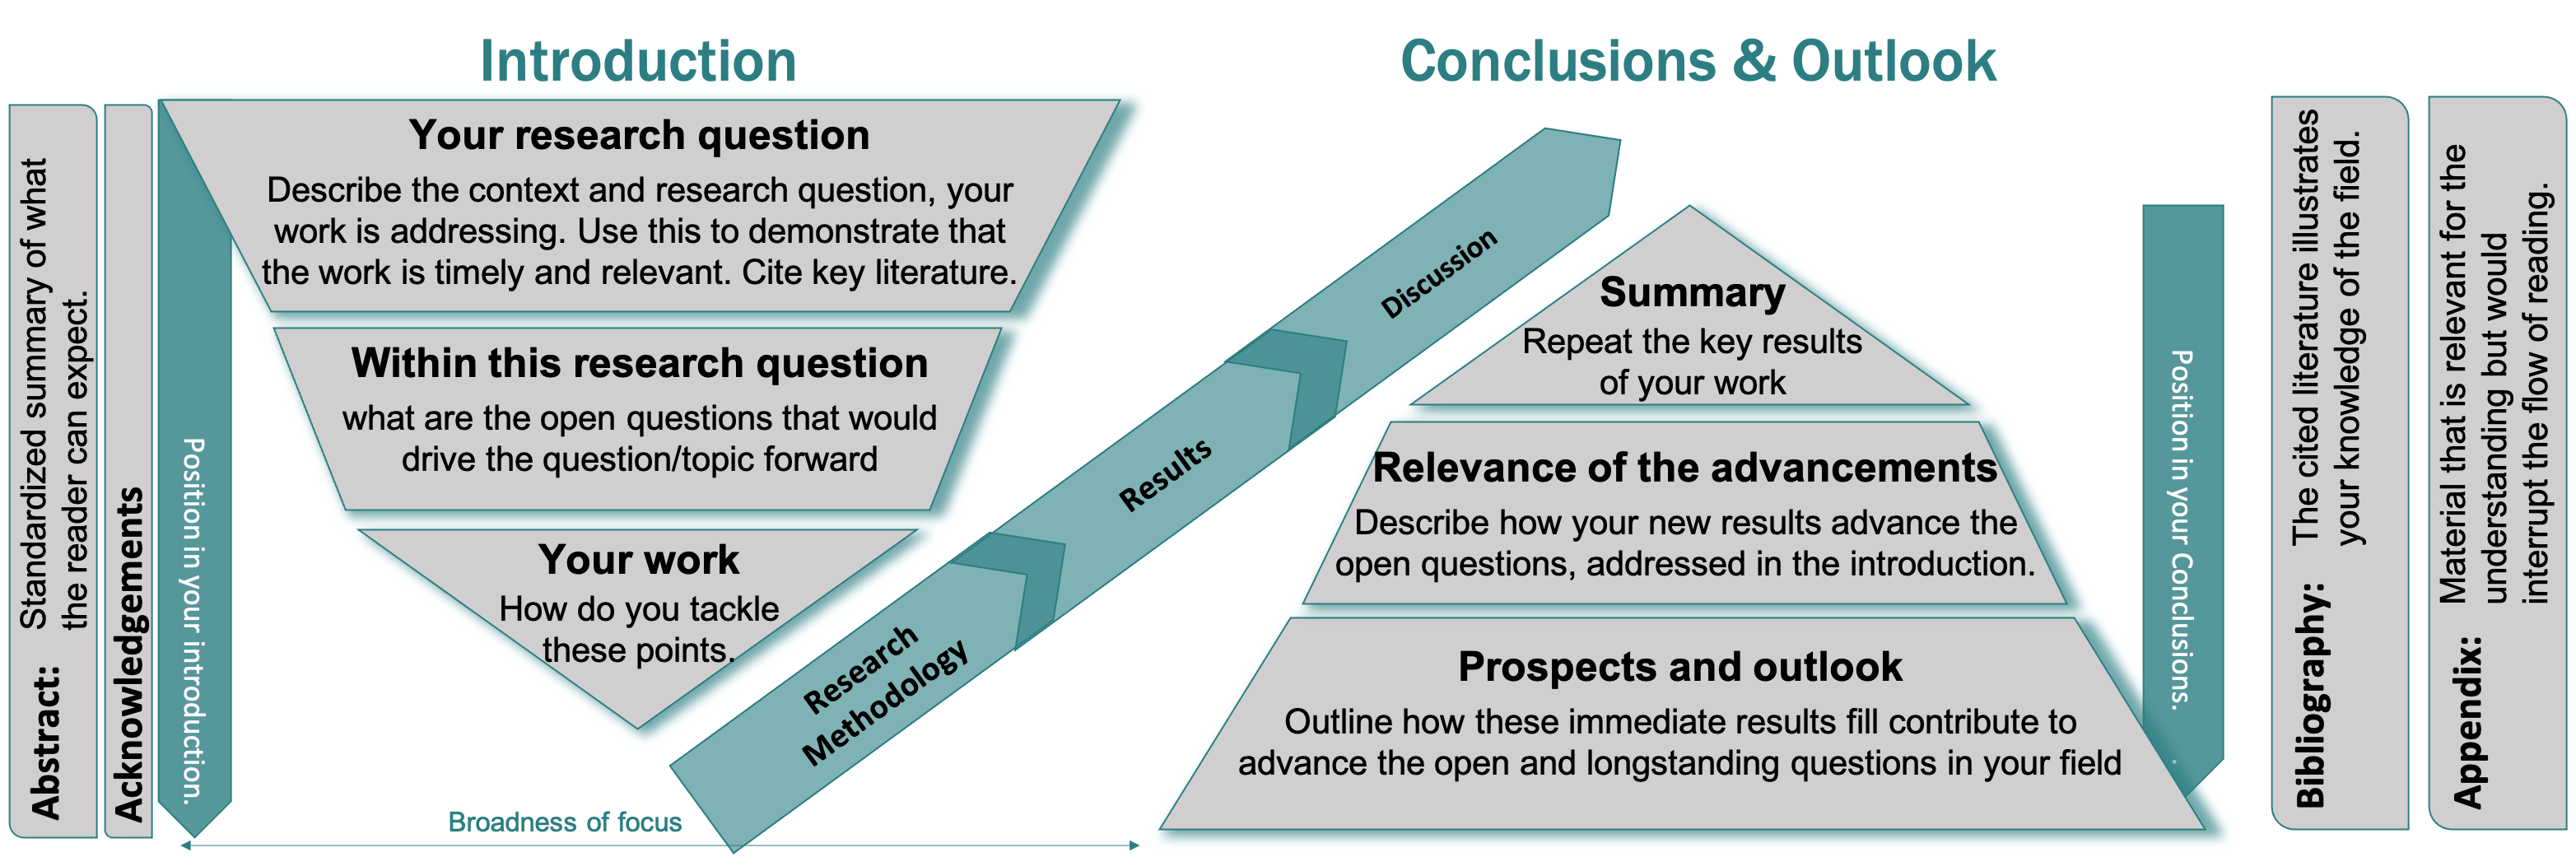
\includegraphics[width=\textwidth]{gfx/constructionMap.png}
    \caption{Schematic structure of the elements of a thesis or research paper. The cones depict the ideal logical flow of the chapters of the \textit{Introduction} and \textit{Conclusions \& Outlook}. }
    \label{fig:logicalFlow}
\end{figure}

%The logical flow of a thesis is illustrated in \Fig{fig:logicalFlow}.
As the first step in your writing process, we recommend that you lay out the anticipated structure and approximate content by crafting chapter and perhaps the main section titles. This first structure can already be implemented in the template and be discussed with your adviser early on. Doing this will allow you to have a more straightforward path to assess the thesis's content and expected workload.


\subsection*{Literature references \& managing your bibliography}
\begin{itemize}
    \item A citation is needed whenever a bibliographic reference to published content is required. The leading astronomical journals use the style of inter-textual citations. In this format, you see the first author's name in the text, most likely to be followed by \textit{et al.} to indicate that more than two authors have signed the paper and the publication year of the paper. The \textit{Bibliography} section in the rear provides all the information on how to retrieve the cited article. Each item listed in the bibliography needs to \hbox{be referenced at least once in the paper.}
    
    \item BibTex is a powerful software package that will help you to easily manage your bibliographic references and the respective bibliography. By using the citation commands 
    $\backslash$cite\{\}, 
    $\backslash$citep\{\}, 
    $\backslash$citep[]$\{\}$, and 
    $\backslash$citep[][]\{\} you create inter-textual references. The following examples show how the above mentioned macros can be used in the syntax of a sentence: 


    
     $-$ \textit{It was shown by \cite{Beck2015} that the long-periodic variations of the radial-velocity signal of $\theta^1$\,Tau originates from stellar activity.} \\
     $-$ \textit{Combining remote-sensing image data with in-situ measurements have lead to an improved flare-CME characterization 
     \citep{Temmer2017}.}\\
     $-$ \textit{The extreme-ultraviolet Radiation from A-stars has significant implications for the formation of \citep[and references therein]{Fossati2018}.}\\
     $-$ \textit{This topic has been discussed in the recent literature
    \citep[e.g. see][and references therein]{Hanslmeier2018phsabook,Veronig2020}.}
    
    \item To cite from a monography use the $\backslash$citep[]\{\} command to reference the book you are citing. If of relevance you can note to which chapter or page you are referring to in the squared brackets of the makro.

    \item Those macros access the content of the file \textit{bib-refs.bib}. To add references, copy the content from \textit{'export citation'} on the NASA ADS webpage of a paper into the bib-file. Experience has shown that it will improve the readability of your  \LaTeX\ code if you change the predefined bibcode (e.g., 2017SoPh..292...93T) into a more user-friendly keyword (e.g., Temmer2017), which is then used in the macros mentioned above to cite the paper.

\end{itemize}

\subsection*{Cross references to elements inside your thesis}
\begin{itemize}
    \item Each Figure, Table, and Equation presented in the paper needs to be referenced at least once in the text body. The objects of each group (figures, tables, equations) must be introduced in the paper in consecutive order: Reference Fig.\,1 in the text before you mention Fig.\,2.
    
    \item Abbreviate the following expressions unless they appear at the beginning of a sentence:  \textit{Sect., Sects., Fig., Figs., Col., Cols.}. \textit{Table} and \textit{Listing} are never abbreviated in a paper. Write the object abbreviation in the upper case if used as a numbered reference. Otherwise, object names should not be abbreviated and written in lower case.
    
    $-$ \textit{\Figure{fig:singelPanelPlot} shows the position of 18 eccentric binary in the HR diagram.}\\
    $-$ \textit{As shown in \Fig{fig:singelPanelPlot}, the 18 eccentric binary are found on the low-luminosity red-giant branch (RGB).} \\
    $-$ \textit{The 18 eccentric binary are found on the low-luminosity RGB (see \Fig{fig:singelPanelPlot}).}
    
    \item To generate an automated numbering, you need to create a reference-able label, using \textit{$\backslash$label$\{$keyword$\}$}. Calling the keyword through the reference macro, \textit{$\backslash$ref$\{$keyword$\}$} will create the reference in the text. You can freely choose the keyword. Experience has shown that it is good practice to encode what kind of object you are referencing into the keyword, e.g.
    \textit{$\backslash$label$\{$fig:HRD$\}$}, 
    \textit{$\backslash$label$\{$tab:redGiantCatalogue$\}$}, 
    \textit{$\backslash$label$\{$eq:pythagoras$\}$}, or
    \textit{$\backslash$label$\{$sec:introduction$\}$}.

    Note that the template contains customized macros in the \textit{main.tex} for all full and abbreviate element names. This way, you only need to type, e.g. \textit{$\backslash$Fig\{fig:HRD\}}, instead of \textit{Fig.$\backslash$,$\backslash$ref\{fig:HRD\}}


\end{itemize}


%\newpage
\subsection*{Figures}
\noindent
Example of single and multi-panel figures and their caption format are given in Fig.\,\ref{fig:singelPanelPlot} and Fig.\,\ref{fig:multiPanelPlot}, respectively.
\begin{itemize}

    \item \physbf{Position:} to be placed on top of the page, using the figure attribute~\textit{[t!]}. Do not place a figure on the first page of a chapter.

    \item \physbf{Message:} be clear to yourself, what take away message is, which you want to give to the reader of your paper by showing this figure. Now optimize your figure to maximize the storytelling: use different symbols, line styles, and colors. A good test for a colored figure is if it is still readable on a black-and-white printout.

    \item \physbf{Caption}: The first sentence of the figure's caption should be a sentence describing the figure. This sentence should start without 'The' / 'This', 'A / An',  or similar.
    Describe all symbols and line styles used in the figure. Express no physical or scientific interpretation of the depicted context.
    
    \item Refer to the figure's axes as the \textit{'horizontal'} and the \textit{'vertical axes'}, instead of the x- and y-axis, respectively.
    
    \item For multi-panel figures, you should refer to the individual panels by using \textit{'top left panel'}, \textit{'middle bottom panel}, or \textit{'bottom right panel'}. 
    
    \item In case you show additional figures depicting different data but using the identical symbol and color scheme, you can refer to the first figure explaining the meaning. State something like \textit{'Meaning of the colors and symbols is similar to Fig.\,XY'}.
        
    \item If you show a figure previously published in another article, you need to indicate the source, such as \textit{(Figure taken from REFERENCE)}. In case somebody provided you  an unpublished figure, you would state  \textit{(Figure provided by PERSON).}    
    
    \item \physbf{Axis labels}: produce plots with readable axes, labels, and ticks. Unreadable labels are the easiest way of getting into \hbox{trouble with the referee (or adviser).}
    

    \item Format: preferably use PNG to avoid excessive file sizes for figures depicting many datapoints.
    

    
\end{itemize}

%\newpage
\subsection*{Tables}
\noindent
An example of a simple, complex and a multi-page table are given in Tab.\,\ref{tab:false_positives}, Tab.\,\ref{tab:asteroseismicValues}, and Tab.\,\ref{tab:longTable} respectively.

\begin{itemize}
    \item \physbf{Position:} to be placed on top of the page, using the table attribute~\textit{[t!]}. Do not place a table on the first page of a chapter.%(The only exception are tables depicting a code's functions, as shown in Appendix\,\ref{chap:appendixCode}.)
    
    \item \physbf{Caption:} (on top of the table): The table caption should be a one-line sentence, describing the table and placing it into the work or paper context. This sentence should start without 'The' / 'This', 'A / An', or similar.
    
    \item \physbf{Layout:} Tables start from above with a double vertical line, followed by the table header, followed by a single line, followed by the table's content. A final horizontal line is closing the table. 
    
    If appropriate, you can use horizontal lines in the table body to mark separations. In this case, the A\&A guidelines refer to the separated blocks as panels. An example is given in  Table\,\ref{tab:false_positives}.
    
    \item The content of the table is typically formatted to the left or right of the column. If you wish to do the extra work for a nice looking table, you can center the header, as shown in Tab.\,\ref{tab:asteroseismicValues}.

    \item \physbf{Tablefoot:} (text block below the actual table starting with \physbf{Notes.}) should contain all relevant information for each column should be provided in the table foot. If you use abbreviated references, you should give the connection to the inter-textual references here. Express no physical or scientific interpretation here. The tablefoot-macro requires an empty line between the text and the table to avoid layout issues.
    
    \item \physbf{Extensive tables} can be presented in the landscape format and / or be split over several pages (longtable). Consider placing it in the Appendix. In this case, you could place the tablefoot-block into the text body of the Appendix as demonstrated in Appendix\,\ref{chap:appendixExtensiveTables}
    
    \item Tables are usually not used in the Introduction or Conclusions chapter.
\end{itemize}

%\newpage
\subsection*{Equations}
\begin{itemize}
    \item Treat equations as part of the sentence and place them like a subordinate clause. See Eq.\,\ref{eq:pyth1}\,and\,\ref{eq:pyth2} for an example.

    \item All mathematical symbols used in the equation need to be defined near the equation, if not defined before in the text. Mention the physical units of the parameter used in the equation.
    
    \item Text in equations or math mode is written in italics per default. In case you want to place a subscript text, which is not an index, you need to force it to be non-italic, e.g., P$_{\mathrm{orb}}$.
    
    %\item multiple equations (if \&=\&, alingement of equations)
    
    %\item \ref{eq:pyth1}, \ref{eq:pyth2} 
\end{itemize}


\subsection*{Presentation of code and code snippets}

One of the bricks of the fundament of science is the replicability of disseminated results. Therefore, the modern standard of research journals that any elaborated code that is used for the data analysis presented in the paper should be made available to the reader. Such code is typically distributed on pages such as GitHub.com. 
For your thesis, we simulate such public distribution of code by presenting your code in the appendix. Discuss with your adviser if or what part of your code should be part of the thesis work. \Listing{code:tidalSettings} and Appendix\,\ref{chap:appendixCode} demonstrate how code (snippet) or pseudo-code is to be presented in the textbody and appendix your thesis, respectively.

\noindent
\physbf{\bfseries\sffamily Presentation in the text body}
\begin{itemize}
    \item Only essential code parts or concepts (via snippets or pseudo code, respectively) should be presented in the main body of your thesis. 
    
    \item The \texttt{verbatim} command is a very severe command, which cannot be used within the iteration tools. Instead of \texttt{verb} or \texttt{verbatim}, please use \textit{$\backslash$texttt$\{\}$}.
    
    \item Treat the code listing like a table. The  \physbf{caption} should be a one-line sentence, describing the table and placing it into the work or paper context. This sentence should start without 'The' / 'This', 'A / An', or similar. Explain the environment and variables in the \physbf{tablefoot}. See \Listing{code:tidalSettings} for an example.
\end{itemize}

\noindent
\physbf{\bfseries\sffamily Presentation in the Appendix}
\begin{itemize}

    \item Before listing the code, provide a preamble outlining your system dependencies of your code (scripting language, version, etc.) Any necessary information should be given in the preceding preamble.
    An expamle is shown in Appendix\,\ref{sec:SystemDependencies} and \Table{tab:PyModules}.
    
    \item Provide a caption as described above, to create a referencable object.
    
    \item Each program should be listed in a separate section of the Appendix. Before listing the source code, provide an abstract of the tasks and functions of the program. Also, give a brief characterization (name, version, download information) of any non-standard package that you have used imported and~used. 
    
    \item \Listing{cod:helloWorld} provides an example. For the reader's benefit, provide in-code comments and documentation.% to make your code to make it more accessible.
    
    \item If you have built-in options, provide a table explaining the options' functionality and how they are called. \Table{tab:functionalityTable} provides an example for the necessary documentation. For those tables, use the positioning argument [h!].
    
    \item To see how to include MESA inlists, activate Appendix\,C. For those use 'language= Fortran'.
\end{itemize}


\subsection*{Abfassen einer Arbeit auf Deutsch}
\begin{itemize}
    \item Sollten Sie diese Arbeit auf Deutsch verfassen, so sind auch die Elemente auf Titelseite, Elementnamen (Abstract, Acknowledgements, Table, Figure) sowie der Colophon zu übersetzen. Die Endung 'et al.' verbleibt als solches.
    
    \item Fachbegriffe müssen in ihrer deutschen Übersetzung ausgeschrieben werden, da eine Mischung zwischen Deutsch und English nicht zulässig ist. 
    
    \item Die Erfahrung hat jedoch gezeigt dass es dem Verständnis des Textes zuträglich ist, wenn in Klammer nach der ersten Verwendung eines Begriffes die englische Originalbezeichnung so wie die in der Literatur übliche Abkürzung angegeben wird.
    Geben Sie im Appendix ein Glossar der englischen Fachbegriffe sowie der in der Arbeit verwendeten Übersetzung wieder (siehe das auskommentierte Bsp.\,\textit{ appendix$\_$DeutschesGlossar.tex}). Im Text können die Abkürzungen Verwendung finden, wobei bei der ersten Abkürzung im Text eine Fußnote zu setzten ist um auf die Tabelle im Appendix zu verwesien, z.B:
    
    
    \textit{Der rote Riesensternast (in der englischsprachigen Fachliteratur auch als \textit{red giant branch} oder abgekürzt RGB\footnote{In diesem Text werden der Fachliteratur entsprechend die Abkürzungen des englischsprachigen Fachbegriffes verwendet. Siehe ebenfalls \Table{tab:glossar} im Anhang.} bezeichnet) ist das Stadium des Wasserstoffschalenbrennens. Dieses RGB-Sterne besitzen einen degenerierten Heliumkern.}
    
    
    
   

\end{itemize}



\begin{center}
\vspace{+5mm}
\color{ctgreenblue}\rule[10pt]{0.3\textwidth}{1pt} 
\vspace{-10mm}
\end{center}

\newpage
\section*{Submitting your thesis at the University of Graz}
\noindent
Once your thesis is ready to be submitted, do the following steps:
\begin{itemize}
    \item \physbf{Finalize your manuscript:} in the file  \textit{titlepages.tex}, \\
    %
    %$-$ deactivate the water mark on Page\,$i$ (see file main.tex). \\
    $-$ change the updated date ($\backslash$\textit{today}) on page $i$ and $iv$ to the date of the submission.\\
    $-$ delete the red line on Page\,$iv$ and fill out the actual date of your submission.\\
    $-$ The corporate-design manual\footnote{\href{https://presse.uni-graz.at/de/services/corporate-design/}{https://presse.uni-graz.at/de/services/corporate-design/}\label{fn:KFUcorporateDesignManual}} of the University of Graz has assigned the \physit{blue-green}, you find throughout the thesis. Please make sure that you have deactivated or deleted all other text-coloring macros, except for \textit{$\backslash$physbf$\{\}$} and 
    \textit{$\backslash$physit$\{\}$}.
    
    \item \physbf{Submission of a Bachelor thesis:} Send the final PDF of your thesis at least a week before you final presentation to your adviser(s). At \physit{University of Graz} you also have to upload your thesis to UNIGRAZonline in order to do the mandatory plagiarism check. A detailed description of the upload process can be found  \href{https://nawi.uni-graz.at/de/studieren/informationen-und-formulare-fuer-studierende/einreichen-von-bachelorarbeiten/}{here}. You will receive feedback from your supervisor about the outcome. 
    When your adviser gave you their approval, please provide a signed hard copy of your thesis to (each of) your advisers. We ask you to produce these copies with a thermal and not a spiral binding. 
    
    
    
    \item \physbf{Submission of a Master thesis:} This summary describes the main steps for the formal submission of your Master thesis at the \physit{University of Graz}.
    Detailed instructions are found on the webpage\footnote{\href{https://nawi.uni-graz.at/de/studieren/informationen-und-formulare-fuer-studierende/einreichen-von-diplom-masterarbeiten-und-dissertationen/}{https://nawi.uni-graz.at/de/studieren/informationen-und-formulare-fuer-studierende/einreichen-von-diplom-masterarbeiten-und-dissertationen/}} the University of Graz.
    %
    For submission of a thesis manuscript at the TU Graz, please refer to their webpage\footnote{ \href{https://tu4u.tugraz.at/studierende/mein-studienabschluss/masterarbeit/}{https://tu4u.tugraz.at/studierende/mein-studienabschluss/masterarbeit/}}.
    
    $-$ You first need to \physit{register the title of your thesis in the university systems}. Ideally, you do this in the final stage of your writing process, about one month before the actual submission to avoid unnecessary delays in the process. 
    %
    To file in your thesis title at the dean's Office, download and complete the latest form\footnote{\href{https://nawi.uni-graz.at/de/studieren/informationen-und-formulare-fuer-studierende/bekanntgabe-des-diplom-oder-masterarbeitsthemas/}{https://nawi.uni-graz.at/de/studieren/informationen-und-formulare-fuer-studierende/bekanntgabe-des-diplom-oder-masterarbeitsthemas/}}. You, your advisers and the head of the Physics Institute must sign this form and it has to be submitted directly (in paper) at the Dean's office for study Affairs ("Prüfungsreferat der Naturwissenschaftlichen Fakultät").
    
    $-$ For the \physit{actual submission of your manuscript}, you have to register and upload your final thesis in your personal \textsc{Uni Graz Online} account. After your adviser has confirmed your thesis online, you have to hand in two hard copies of your work (plus a form\footnote{   "Ansuchen um Beurteilung der Masterarbeit oder Diplomarbeit", to be downloaded at  \ref{footnote:MasterPhD}}),
    including the abstract but without the declaration, into the Dean´s office. The electronic upload automatically initiates the obligatory \physit{plagiarism check}. 
    
    For your planning, please consider that it takes \physbf{at least four weeks} (from the submission of your thesis) before your the date of the Master´s exam can be scheduled. After your adviser has officially graded your thesis, you are done with your thesis. 
    
    Detailed instructions and up-to-date forms for the submission process of master and PhD thesis can be found on the webpage\footnote{\label{footnote:MasterPhD} \href{https://nawi.uni-graz.at/de/studieren/informationen-und-formulare-fuer-studierende/einreichen-von-diplom-masterarbeiten-und-dissertationen/}{https://nawi.uni-graz.at/de/studieren/informationen-und-formulare-fuer-studierende/einreichen-von-diplom-masterarbeiten-und-dissertationen/}} the University of Graz.
    
    For the submission of a thesis of students who are main inscribed at the TU, it is important that you replace \physit{'titlepageKFU.tex'} with \physit{'titlepageTU.tex'} and adapt it accordingly.
 
 \item \physbf{Submission of a PhD thesis:} Detailed instructions and up-to-date forms for the submission process of a PhD thesis are found on the webpage$^{\ref{footnote:MasterPhD}}$ of \hbox{our Alma Mater, the University of Graz.}
\end{itemize}


\newpage
\section*{Color scheme and implemented tools for iteration}
\noindent The implemented blue-green color in section headings and text markup agrees with the corporate-design manual$^{\ref{fn:KFUcorporateDesignManual}}$ of the University of Graz and the assigned scheme for the Institute for Physics. You can use these comments to highlight important text. This is the only color to be used for text as \hbox{markup in the submitted version.}
\begin{table}[h!]
    %\centering
    \hfill\begin{tabular}{p{0.25\textwidth}p{0.70\textwidth}}
    \hline\hline
    Macro name & Example \& Explanation \\[0.5em] \hline
    
    %-----------------------------------------------------
    %Corporate Identity 
    
    \smallskip
    \textit{$\backslash$physbf$\{\}$}  & 
    \smallskip \physbf{bold text with CI color.} \\[0.5em]
    
    \textit{$\backslash$physit$\{\}$} &
    \physit{italic text with CI color.}\\[0.5em]
    \hline
    \end{tabular}
    \hfill~
    
\end{table}

\vspace{-5mm}
You will find the following macros useful to mark text or place action items and comments in the iteration phase. This approach adopts typical elements of a paper's revision phase, indicating changes requested by the referee. 
\begin{table}[h!]

    %\centering
    \hfill\begin{tabular}{p{0.25\textwidth}p{0.70\textwidth}}
    %\hline\hline Macro name & Example \& Explanation \\[0.5em] 
    \hline
    
    %-----------------------------------------------------
    
    \smallskip \textit{$\backslash$myComment$\{\}$} &    
    \smallskip \myComment{Macro marking a comment with your initial.}\\[0.5em]
    \textit{$\backslash$myRevision$\{\}$} &
    \myRevision{This macro is to mark text, revised according to your adviser comment.}\\[0.5em]
    \textit{$\backslash$myToDo$\{\}$} &
    \myToDo{describe your identified action item.} \\[0.5em] \hline 
    \end{tabular}
    
    \hfill~
    
\end{table}

\vspace{-5mm}
If you and your adviser choose to communicate via a shared project on overleaf, then your adviser has the following defined tools at their disposal to mark and comment.  Typically, you can expect an explanation next to \textit{Markover} or \textit{Cossout} why this text requires further attention or should be deleted.
\begin{table}[h!]
    %\centering
    \hfill\begin{tabular}{p{0.25\textwidth}p{0.70\textwidth}}
    %\hline\hline Macro name & Example \& Explanation \\[0.5em] 
    \hline
    
    %-----------------------------------------------------
    
    \smallskip \textit{$\backslash$adviserComment$\{\}$}  &\smallskip\adviserComment{Macro marking a comment of your adviser}\\[0.5em]
    
    \textit{$\backslash$adviserAddition$\{\}$}  &\adviserAddition{Macro marking an textual addition to your thesis.} \\[0.5em]
    
    \textit{$\backslash$adviserHighlighted$\{\}$}  &\colorbox{yellow}{\parbox{0.7\textwidth}{Macro highlighting a text in yellow.}} \\[0.5em]
    \textit{$\backslash$longSentence$\{\}$}  &\colorbox{yellow}{\parbox{0.7\textwidth}{Same as above, printing \textit{'long sentence'} to the right.}} \\[0.5em]
    
    \textit{$\backslash$adviserMarkover$\{\}$}  &
    \adviserMarkover{Macro marking a text that requires a makeover.}\\[0.5em]
    
    \textit{$\backslash$adviserMarkoverComment$\{\}\{\}$}  &
    ~~~~~~~~~~~~~~\adviserMarkoverComment{Marking text.}{Placing a comment}\\[0.5em]
    
    \textit{$\backslash$adviserDelete$\{\}$}  &\adviserDelete{Text to be deleted.}\\[0.5em]
    \hline
    \end{tabular}
    \hfill~
    
\end{table}

\vspace{-5mm}
You are free to change the iterative tools' color settings if you do not like the chosen colors. If so, please make sure that your and your adviser's macros remain well distinguishable in color.

%Note on writing in German: Sofern in Deutsch geschrieben wird wäre es hilfreich wenn dennoch die Abkürzungen aus der englischen Fachliteratur verwedent würden. Um konsistent zu bleiben, bietet sich folgende erklärenden Fußnote bei dem ersten Fachbegriff an, z.B. 
%"Die Leuchtkraft eines Sternes an der Spitze des roten Riesenastes (in der englischsprachigen Fachliteratur auch als \textit{red-giant branch} oder abgekürzt\footnote{In diesem Text werden der Fachliterature entsprechend die Abkürzungen des englischsprachigen Fachbegriffes verwendet} als RGB bezeichnet.) von bestimmten Parametern abhängt und beeinflusst wird. % read me before starting to write. Not part of the actual deliverable.


\pagestyle{plain}				% display just page numbers
\begin{titlepage}
    \centering
    \vspace{8cm}
    {Bachelor Thesis \par}
    
    {\scshape\LARGE Adsorption of Organic Molecules on Ag(100) and MgO(100)/Ag(100) \par}
    
    \vspace{3cm}
    {\large For the attainment of the degree Bachelor of Science (B.Sc.) \\ from the Institute of Physics at University of Graz. \par } 
    {\large Aleksey Sokolov  \par}
    {\large Matr.: 12004091 \par}
    \vspace{5cm}
    \vfill
    {
\includegraphics[width=3.5cm]{Uni_Graz.PNG}\par}
    
    
    {\large Supervisor: Univ.-Prof. Sterrer \par}
    
    {\large Graz, September 2023\par} 
\end{titlepage}
\chapter*{Abstract}
\label{sec:abstract}


% ------------------------------------
\cleardoublepage
%
\setcounter{tocdepth}{2}		% define depth of toc
\tableofcontents				% display table of contents
\cleardoublepage

% --------------------------
% Body matter
% --------------------------
\pagenumbering{arabic}			% arabic page numbering
\setcounter{page}{1}			% set page counter
\pagestyle{maincontentstyle} 	% fancy header and footer
%Include various chapters that are in the folder content


%***************ANMERKUNGEN*******************
\chapter{Introduction}
\label{sec:anmerkung}
The study of molecular adsorption on solid surfaces is an important and influential field within surface science.
This thesis is a comprehensive exploration of the adsorption behaviour of two organic molecules, Pentacenequinone (PQ) and 2 Hydrogen Phtalocyanine (2HPc), on Ag(100) and MgO(100)/Ag(100).
The present study delves into the phenomenon of Fractional and Integer Charge Transfer (FCT and ICT) and the formation of ordered structures. 
Organic molecules with semiconductive properties such as 2HPc, exhibit significant potential in opto-electronic technologies.
The enhancement of device efficacy and functionality is reliant on their surface interactions. 
Furthermore Phthalocyanines are used as enzyme-like catalysts , liquid crystals, in photovoltaic cells or as photodynamic reagents for cancer therapy. \cite{wang2012structures}
The versatility of these molecules arises from their ability to form coordination complexes with metals, giving them the name Metal-Phthalocyanines (MPc).\cite{wang2012structures}
This process can change their optical or electronic properties, while leaving the inherent geometric structure unchanged \cite{wang2012structures}.
Hence, it is important to understand the intricacies of their adsorption behavior, charge transfer mechanisms, and structural order formation to achieve technological progress. \\
%It was even shown for a similar group of organic molecules the porphyrins, to be precise 2H-tetraphenylporphyrin (2H-TPP), that the self-metallation on thin MgO films can occur.
%This process called metallation is promoted by charge transfer and can be controlled by tuning the work function of the MgO(100)/Ag(100) subtrate \cite{egger2021charge}.
%Therefore something similar for 2HPc is expected.
For 2H-tetraphenylporphyrin (2H-TPP), a molecule similar to 2HPc, self metallation has been observed on MgO(100) thin films. \cite{egger2021charge}
Interestingly, in this case charge transfer seems to play a crucial role in this process.
In 2H-TPP the 4 peripheral phenyl rings are tilted relative to the plane of the molecular macrocycle, leading to a relativly high adsorption height of the macrocycle .
Charge transfer transfer reduces this adsorption height, enabling self metallation (see Fig. \ref{fig:2htpp}).
\monofig{width=0.7\textwidth}{2http.jpg}{Selfmetallation precess of 2H-TPP on MgO(100)/Ag(100) \cite{egger2021charge}}{fig:2htpp}
Naturally, this leads to the question whether those two processes, self-metallation and charge transfer, are also connected in such a way for completely flat molecules, such as 2HPc.
The aim of this thesis is to understand and categorize the adsorption behavior of both
adsorbates on an Ag(100) single crystal and on a MgO(100) thin film grown on
Ag(100), with the main focus on 2-Hydrogen-Phthalocyanine (2HPc).
PQ is exclusively imaged on Ag(100), where the focus is to observe bigger structures without imaging individual molecules.




%********VORAUSSETZUNGEN & GRUNDLAGEN*********
\chapter{Fundumentals}
\label{sec:Fundumentals}
\section{STM-Imaging}
The Scanning Tunneling Microscope was introduced in 1981 by Gerd Binning and Heinrich Roherer. 
With this measuring technique it is possible to resolve a conductive surface with a precission beyond that of conventional light based Microscopes.
In contrast to other electron based microscopy like Scanning Electron Microscopes (SEM) it uses the quantum mechanical phenomenon of tunneling.
In classical mechanics, objects cannot overcome a potential if their energy $E < V_0$, as observed in gravitational interactions.
This phenomenon is observed for quantum mechanical particles like electrons, which can surpass a potential barrier despite the initial expectation that they should not be able to.
The STM uses this effect by precisely positioning a sharp conductive tip close to the surface and applying a bias voltage.
Most STM are operated in Ultra-High-Vacuum (UHV), where the distance between the tip and the surface represents the tunneling barrier.
By varying the bias voltage, the tunneling probability can be changed, thereby affecting the tunneling current.
If the bias voltage, also referred to as the potential difference, is kept constant, the tunneling current is primarily dependent on the distance between tip and surface.
The tip is moved in the x-,y-plane where a grid is established. 
There are two modes of operation, the constant-height and the constant-current mode.
The latter is especially useful for irregular surfaces, because the tip is moved up and down to keep the tunneling current constant.
The movement signal of the piezos is then converted into height.
In constant-height mode the position of the tip stayes fixed and the tunneling current $I_t$ is measured and converted into height information. \\

\newpage
\begin{wrapfigure}{r}{0.5\textwidth}
    \centering
    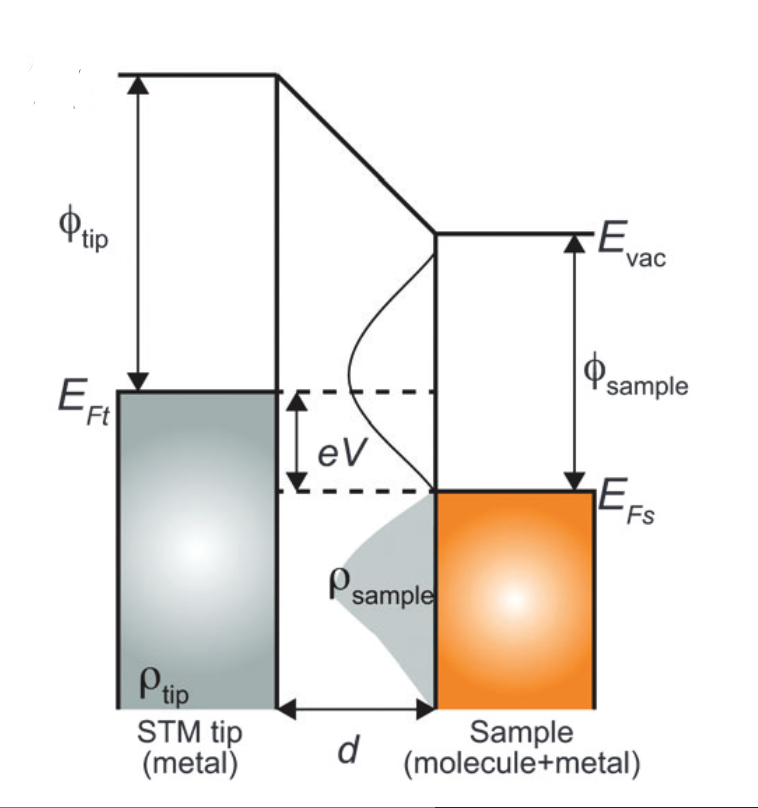
\includegraphics[width=0.4\textwidth]{graphics/Tunneling_diagram_japan.PNG}
    \caption{Energy diagram of the tunneling  junction with a positive bias voltage applied. $\Phi_{tip}$ \& $\Phi_{sample}$: working functions of either tip and sample, $E_{vac}$: vacuum energy level,  $E_{ft}$ \& $E_{fs}$: Fermi Energys of the tip and sample,  $\rho_{tip}$ \& $\rho_{sample}$: density of states of tip and sample,  $eV$: potential difference caused by applying a bias Voltage $V$ (picture source: \cite{Kano}) }
    \label{fig:energy_diagram}
\end{wrapfigure}

The tunneling current, at a arbituery gridpoint, is influenced by the electronic structure of the tip and sample.
If the tip is in vicinity of the metallic substrate the fermi energies align, resulting in an equal probability of electrons tunneling from the tip to the sample and vice versa.
This consequently results in a zero net current. 
Through the introduction of a electric potential $V_{bias}$ the fermi energies of tip and sample can be shifted relative to each other (Figure \ref{fig:energy_diagram}).
If the bias voltage is positive the fermi energy of the sample is pushed down and electrons from occupied states in the tip can tunnel into the empty states of the sample.
Consequently if the bias voltage is negative electrons from the filled states of the sample tunnel into the tip.
The tunneling current is influenced by the distance $d$ between orbitals of the tip and the sample, which makes it possible to gain information about the electronic structure of the sample.
This is not really a representation of the real structure of the atoms or molecules, but the Local Density of States (LDOS) of the sample´s surface.
Utilizing this in Scanning Tunneling Spectroscopy (STS) provides additional information beyond the sample's topography.
Such as the chemical composition, bonding, the energy gap and band-bending effects [\cite{cbai}].
\newpage
\section{Mathematical Foundation STM}

To understand the tip sample interaction one must look at the quantum-mechnical Foundation behind it.
At its simplest the tip can be approximated as spherical potential well (Figure \ref{fig:tip_scheme}). $R$ is in that case the radius of the tip located at position $\vec{r_0}$ with the distance $d$ from the surface.
First order pertubation theory gives the following expression (Eq. \ref{eq:tunneling_pert}) for the tunneling current of this system [\cite{PhysRevLett}]:
\begin{equation}
    I = \frac{2 \pi e}{\hbar} \sum_{\mu \nu} f(E_{\mu})[1 - f(E_{\nu}+eV_{bias})]\cdot |M_{\mu \nu}|^2 \delta(E_{\mu}- E_{\nu})
    \label{eq:tunneling_pert}
\end{equation}\\

\begin{wrapfigure}{r}{0.3\textwidth}
    \centering
    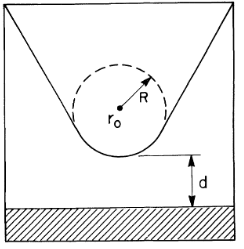
\includegraphics[width=0.3\textwidth]{graphics/fundamental_tip_sheme.PNG}
    \caption{Schematic depiction of the tip geometry [\cite{PhysRevLett}]}
    \label{fig:tip_scheme}
\end{wrapfigure}

\noindent The fermi distribution $f(E)= (\exp((E-E_F)/k_b T)+1)^{-1}$ gives the ocupation probability of a fermion (electrons) with the Energy $E$ near the fermi level.
In this case it is the ocupation probability of the tip states (denoted by the subindex $\mu$) and the ocupation probability of the sample states ( denoted by the subindex $\nu$).
The tunneling matrix $M_{\mu \nu}$ is related to the derivatives of the sample wave functions $\psi_{\nu} $ at the nucleus of the apex atom [\cite{tunnelmatrix}].
Because the STM Imaging is done at low temperatures and with small voltages the Equation \ref{eq:tunneling_pert} can be simplified to:
\begin{equation}
    I = \frac{2 \pi}{\hbar} e^2 V_{bias} \sum_{\mu \nu}  |M_{\mu \nu}|^2 \delta(E{\nu}-E_F) \delta(E_{\mu}- E_{F})
    \label{eq:tunneling_pert_simple}
\end{equation}
With the tunneling matrix $M_{\mu \nu}$ , which relates to the probability of an electron transitioning from state $\mu$ to state $\nu$ [\cite{tunnelmatrix}]: 
\begin{equation}
    M_{\mu \nu} = \frac{\hbar^2}{2m} \int (\psi_{\mu}^{*} \vec{\nabla} \psi_{\nu} - \psi_{\nu} \vec{\nabla} \psi_{\mu}^{*}) \, d\vec{S}
    \label{eq:tunnelin_matrix}
\end{equation}
To obtain a solution  , the tip wave function can be explicitly chosen as an s-type orbital, this holds true for a tungsten tip as it has a only a s-type orbital occupied in its valence shell.
This orbital has a spherical form [\cite{PhysRevLett}]:
\begin{equation}
    \psi_{\mu} = \Omega_t^{-1/2} * c_t k R e^{kR} ( k|\vec{r}- \vec{r_0}|)^{-1} e^{-k|\vec{r}- \vec{r_0}|}
    \label{eq:tip_wave}
\end{equation}
$\Omega_t^{-1/2}$ is the volume of the probe, $k = \hbar^{-1} \sqrt{2m\phi}$ is the inverse dacay length for the wave functions in vacuum, $c_t$ is a geometry specific constant on the order of 1 and $R$ is the radius of curvuture.
The surface wavefunctions can be approximated as blochwaves, which are plane waves modulated by a periodic function.
In the region of neglible Potential the surface wavefunction can be written as:
\begin{equation}
    \psi_{\nu} = \Omega_{s}^{-1/2} \sum_{G} a_G \exp(- (k^2 + |\vec{k}_{||} + \vec{G}|^2)^{1/2} z)\cdot \exp(i(\vec{k}_{||} + \vec{G})\cdot \vec{x})
    \label{eq:surface_wave}
\end{equation}
Here $\Omega_{s}^{-1/2}$ is the sample volume, $k$ the previously mentioned inverse decay length, $\vec{k}_{||}$ is the surface bloch wave vector and $\vec{G}$ represents the reciprocal surface vector.
Substituting into \ref{eq:tunneling_pert_simple} as seen in executed in [\cite{PhysRevLett}] gives the result:
\begin{equation}
    I = 32 \pi^3e^2 V_{bias}\phi^2 D_t(E_F)R^2 k^{-4} e^{2kR} \cdot \sum_{\nu} |\psi_{\nu}(\vec{r_0})|^2 \delta(E_{\nu} - E_F) 
\end{equation}
Where $D_t(E_F)$ is the Density of States of the Tip at the Fermi Level. 
The sum over the local states of the surface $\psi_{\nu}$ at the Fermi Level ($\delta(E_{\nu} - E_F)$) can be interpreted as the Local Density of States (LDOS).
Using the surface wavefunction one can see that the tunneling current is following an exponential decay, that is proportional to the distance $d$ between the tip and the sample:
\begin{equation}
    I \varpropto e^{-2 \cdot d \sqrt{\frac{2m \phi}{\hbar^2}}}
    \label{eq:propcurrent}
\end{equation}




\newpage

\section{Low Energy Electrons Diffraction (LEED)}
A well collimated beam of electrons with the same wavelengh is directed at a flat surface.
In this case the wavelengh of the incoming electrons is determened by the electric field $U_a$ that acts upon them \ref{eq:electron_wavelengh}.
To see diffraction the wavelengh of the electrons must be in the range of the lattice constant, as is effectively show by the concept of the ewald sphere.
Typically the kinetic energy of the electrons is up to $E_{kin} = e U_a = 200$ eV.
\begin{equation}
    \lambda = \frac{h}{\sqrt{2 m_e e U_a}}
    \label{eq:electron_wavelengh}
\end{equation} 
If the surface is periodic this results in a sharp pattern of spots that reflects the k-space of the crystal.

\begin{wrapfigure}{r}{0.6\textwidth}
    \centering
    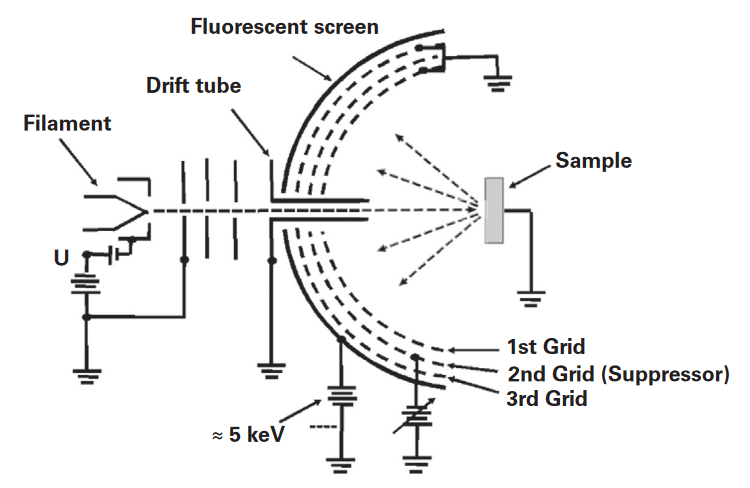
\includegraphics[width=0.5\textwidth]{graphics/fundamental_leed_setup.PNG}
    \caption{A basic three-grid LEED system which utilizes a flourenscent screen as imaging tool \cite{MoritzWolfgang2022SSDb}}
    \label{fig:LEED_Shematics}
\end{wrapfigure}

\noindent The LEED setup consists of a filament which emitts electrons by applying a current.
This electrons are then accelerated and collimated in a drift tube which points at the sample.
Due to interactions of the electrons with the crystal atoms some of them are not diffracted elastically.
To ensure that only the elastically scattered electrons are show on the flourencent screen, a grid system is installed in front of the screen.
The first grid and the sample are both grounded to ensure that the diffracted alectrons propagate undesturbed through the space between the sample and the grid.
A filter Voltage is aplied between the second and third grid that is just below the acceleration voltage.
Electrons which are not elastically scattered are completely stopped, which makes it effectivelly a high pass filter. [\cite{MoritzWolfgang2022SSDb}] \\

\noindent The collimated beam can be represented as a planar wave $e^{i \vec{k_0} \vec{r}}$  outside the surface.
The wavevector $\vec{k_0}$ points in the propagation direction and represents the spacial frequency of the wave.
This vector can be modeled as:
\begin{align}
    |\vec{k_0}| &= \frac{2 \pi}{\lambda} = \frac{\sqrt{2 m_e E}}{\hbar} \\
    \hspace{1cm} \notag \\
    \vec{k_0} &= \begin{pmatrix}
        |k_0|\cos(\varphi)\sin(\vartheta)\\|k_0|\sin(\vartheta)\sin(\vartheta)\\|k_0| \cos(\vartheta)
    \end{pmatrix}
\end{align}
A 2D periodic surfuce structure with a reciprocal basis ($b_1$,$b_2$) causes the plane waves to diffract.
The diffracted waves have the shape $A_g e^{i \vec{k_g} \vec{r}}$ with wave vectors $|\vec{k_g}| = |\vec{k_0}|$.
$\vec{k_g}$ transforms according to $\vec{k_g} = \vec{k_0} + \vec{g}$. 
The reciprocal lattice vector $\vec{g} = 2 \pi ( h b_1 + k b_2)$ represents the individual points where constructive interference is present.
Usually the indices h and k are intergers which characterize the beam, for example (0,0) or (1,1).
It can be shown that the wave vector in vacuum outside the surface is [\cite{MoritzWolfgang2022SSDb}]:
\begin{equation}
    k_g = - \sqrt{\frac{2 m_e E}{\hbar^2} - (k_{0x}+ g_{x})^2 - (k_{0y}+ g_{y})^2}
\end{equation}

%\polyfig{graphics/fundamental_kspace.PNG}{hllohi}{fig:kspace}{graphics/fundamental_kspace_theta.PNG}{fig:kspace_}{helo}

%\begin{figure}[H]
%    \centering
%    \begin{minipage}[b]{0.49\textwidth}
%        \centering
%        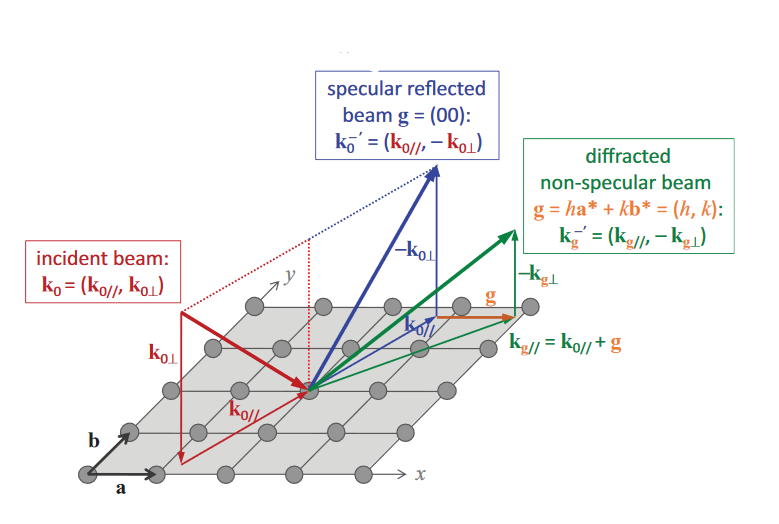
\includegraphics[width=\textwidth]{graphics/fundamental_kspace.PNG}
%        \caption{
%            2D lattice with the reciprocal lattice vectors $\vec{a}$ and $\vec{b}$. 
%            $\vec{k_0}$ (red): incident beam,
%            $\vec{k_{0}^{-}}'$ (blue): specular reflected beam,
%            $\vec{k_{g}^{-}}'$ (green): non-specular diffracted beam, }
%        \label{fig:kspace}
%    \end{minipage}
%    \begin{minipage}[b]{0.49\textwidth}
%        \centering
%        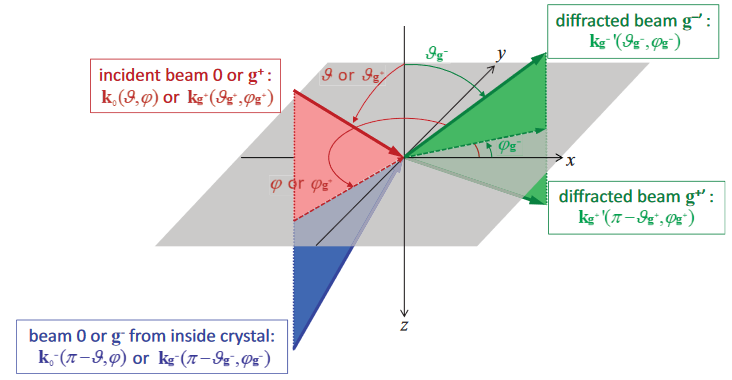
\includegraphics[width=\textwidth]{graphics/fundamental_kspace_theta.PNG}
%        
%        \caption{hgh}
%        \label{fig:kspace2}
%    \end{minipage}
%\end{figure}
%

\duofigcom{graphics/fundamental_kspace.PNG}{fig:kspace}{graphics/fundamental_kspace_theta.PNG}{fig:kspace2}{
    (a): 2D lattice with the reciprocal lattice vectors $\vec{a}$ and $\vec{b}$. 
    $\vec{k_0}$ (red): incident beam,
    $\vec{k_{0}^{-}}'$ (blue): specular reflected beam,
    $\vec{k_{g}^{-}}'$ (green): non-specular diffracted beam, }{}




\section{Adsoption}
\newpage
%************VERSUCHSANORDNUNG*************
\chapter{Experimental Setup}
\label{sec:versuchsandordnung}
The experimental work done in this thesis primarily utilized a Low-Temperature Scanning Tunneling Microscope setup (LT-STM).
This STM is composed of two distinct compartments, the preparation chamber (PC) the measurement chamber (MC).
The sample is inserted through a airlock into the preparation chamber.
In the whole system there is in a Ultra High Vacuum (UHV) at about 10$^{-11}$ - 10$^{-10}$ mbar, which is archieved by four individuall pumps.
The base Vacuum is achieved with the turbomolecular pump and the scroll pump through the airlock.
Additionally there is a titanium sublimation pump and a ion pump in the preparation room.

\monofig{width=\textwidth}{Experimental_Setup/STM_Picture_1_edited.pdf}{
    The experimental setup used, 
    A: cooling-chamber filled with Liquid Oxigen,
    B: measuring-chamber with spring suspended sample holder and tip,
    C: sputter-gun,
    D: metal-evaporater,
    E: molecule-evaporater,
    F: preparation-chamber with free movable sample holder arm,
    G: LEED system,
    H: Electronic used to monitor the function of the STM}{fig:stm_uni_kf}
%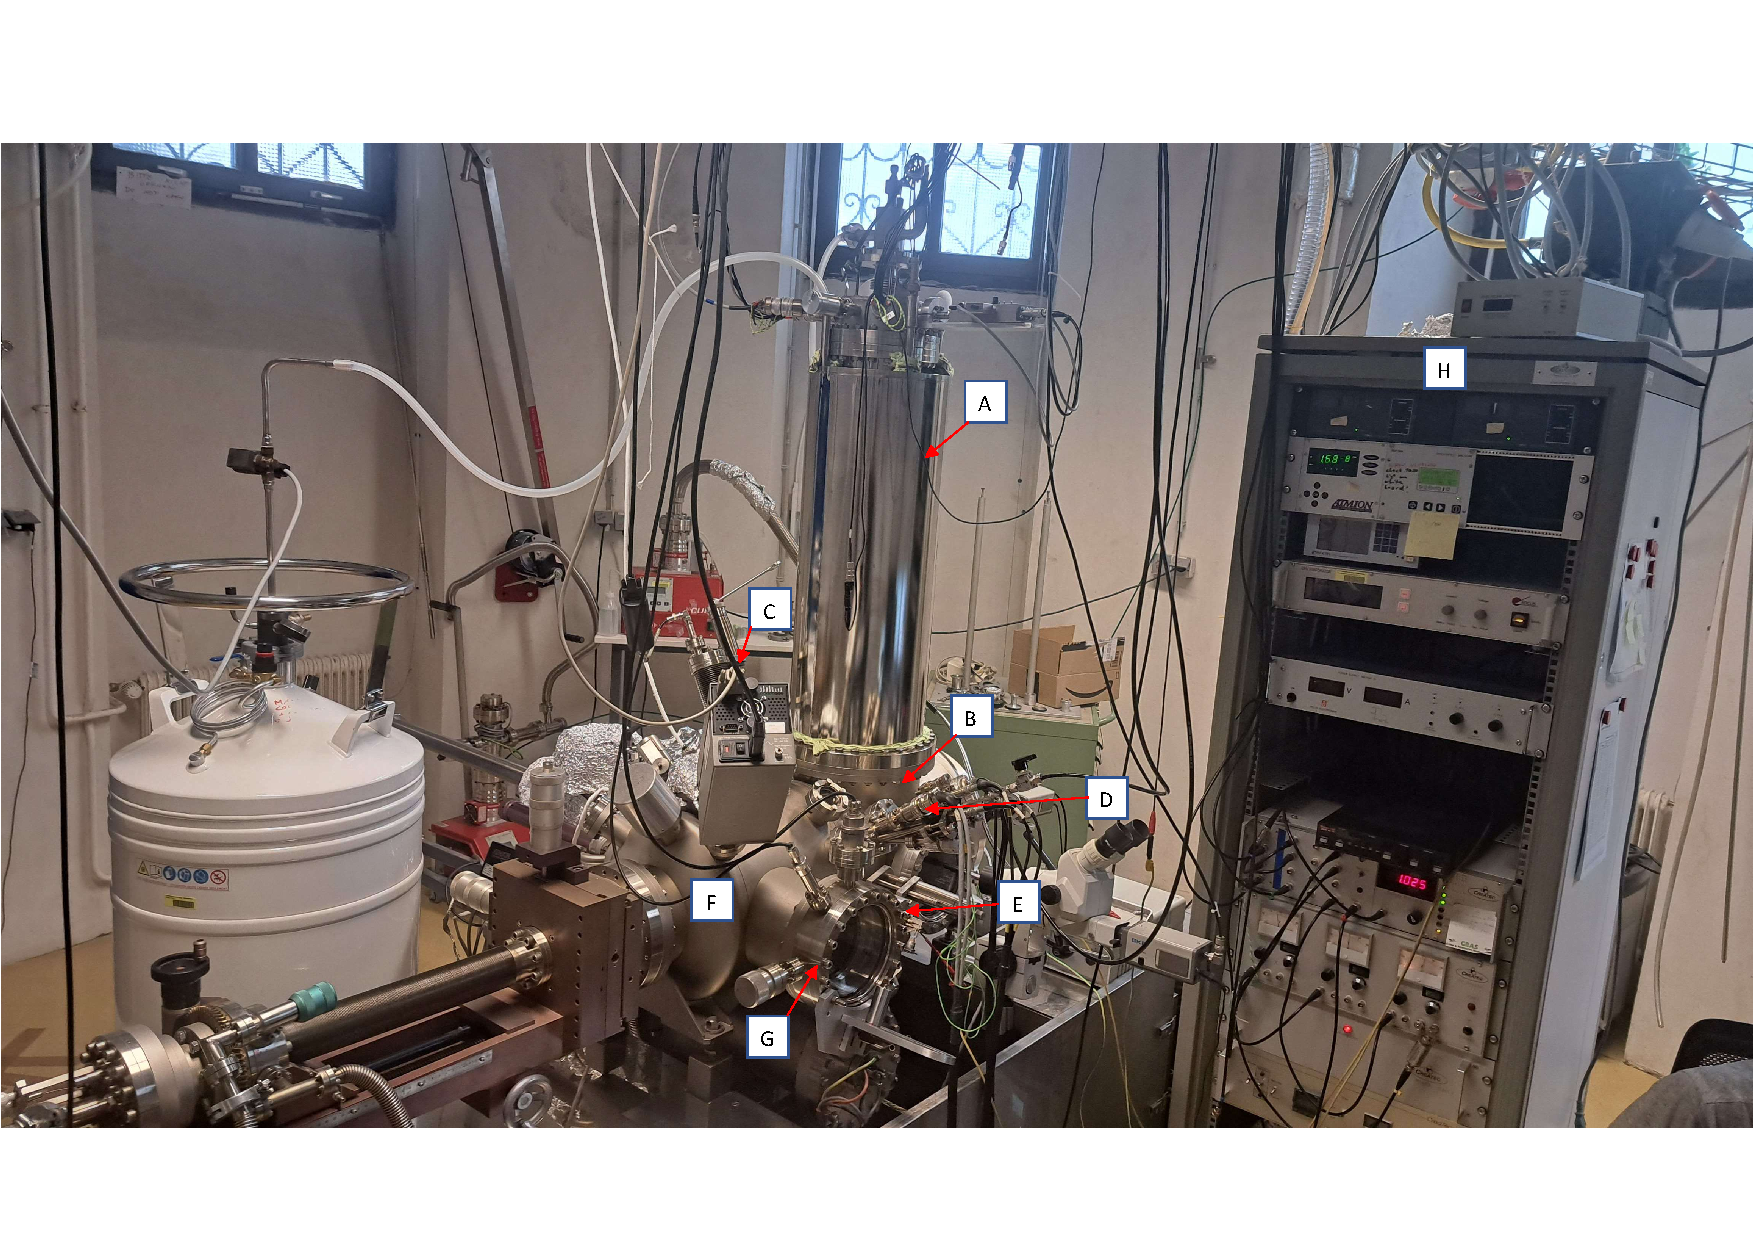
\includegraphics[width=0.9\textwidth]{Experimental_Setup/STM_Picture_1_edited.pdf}

The Probe-holder can be moved in each direction and rotated using an integrated arm in the PC.
It is also used to insert the Probe-holder into the MC.
The PC is equipped with a LEED system, which fluorescent screen can be extended. 
Additionally the PC has a metal-evaporator and organic-molecule evaporator (e-beam evaporator with a triple Knudsen cell) which are used to deposit submono- or monolayer structres onto an circular sample (10 mm x 2 mm).
This sample is mounted onto the previously mentioned Probe-holder, a Heatwaves Labs Inc. button heater with a resistive heating range of 20 K - 900 K.
The sample can also be cooled using LN2 or LHe through built-in pipe system in the manipulator arm.
A Quartz-Crystal Microbalance (QCM) with sub Angstöm precision is used to monitor the deposition thickness.
To clean the sample, an Argon sputter gun is employed, which utilizes an electric field to ionize and accelerate the argon gas.
The MC consists of a LT-STM which is surrounded by a two-shell cryostat, to which it is fixed, and two radiation shields to archieve temperatures as low as 7 K.
In this thesis the cryostat chamber was filled with LN2 which means it was operated at 75 K.
The primary measuring unit (tip and sample storage place) is vibrationally damped using a coupled spring system.


\section{Sample Preparation}
\subsection{Substrate}
The Substrate used in this thesis is a Silver (Ag) single crystal.  
Silver is a metal with 47 Protons and two stable isotopes 107Ag and 109Ag that are almost almost equally distributed.
It has an atomic radius of 1.44 \AA and it naturally crystallizes into a face centered curbic (fcc) structure with a lattice constant of a = 4.079 \AA. [\cite{PhysRev.25.753}]
The single crystal is cut along the (100) plane giving it a square surface lattice along the [011] and [01$\bar{1}$].
This reduces 

\subsection{Pentacene-Quinone}


\subsection{2-Hydrogen Phthalocyanin}
%************AUSWERTUNG****************
\chapter{Results}
\section{Pentacenequinone}
Unfortunately inspite of three attempts to get a stable evaporation process it was not possible to get sub-monolayer/monolayer growth.
This lead to difficulties regarding image resulution,but it was still possible to observe makrostructures forming.
Pentacenequinone seems to form round island that are randomly scattered and have no clear periodic structure.
If looking closely at the edges of the terasses, it is visible that the sharp edges that are typical for Ag(100) are rough.
This could indicate a full monolayer present.
\duofigcom{C:\\Bac_Arbeit\\ratumi_bac\\bac_template\\graphics\\ready_images_pentacene\\41nm_pentacene_3dig.png}{fig:penta_3dig}{C:\\Bac_Arbeit\\ratumi_bac\\bac_template\\graphics\\ready_images_pentacene\\41nm_pentacene_1dig.png}{fig:penta_1dig}{seas}{}

\newpage
\section{2-Hydrogen Phthalocyanin on Ag(100)}
\label{sec:results}The STM and LEED Images of 2-Hydrogen Phthalocyanin (2HPc) on Ag (100) show the Formation of an ordered Structure.
As seen in the Image \ref{fig:2hpcAg_o} the 2HPc  is most likely in $\sqrt{17} \times  \sqrt{17}\text{R}14$ Phase with an relative rotation of the molecular axis (MA) in respect to the [010] direction of 7 ° (see figure \ref{fig_fig:2hpcAg_o}). 
Furthermore the STM Images reveal that the distance between the nearest molecules is 
15 A and that the unit cell of the monolayer is also square.
\monofig{width = 0.7\textwidth}{C:\\Bac_Arbeit\\ratumi_bac\\bac_template\\graphics\\ready_images_phthalo\\2Hpc_on_Ag100_3.PNG}{STM image of 2HPc/Ag(100) taken in constant-current mode (monolayer regime).(a) Constant-height Image of Ag(100) as reference  . U = 53.5 mV , I = 1 nA. MA: Molecular axis.}{fig:2hpcAg_o}  
\noindent The Molecule itself appears as a 4-fold symmetric cross with a dark center in the middle or as 2-fold symmteric cross with two opposing isoindole units seeming brighter than the other two for positive polarity . 
It oriented so that the benezene ring of one 2HPc molucule is pointed towards the benzene ring of the nearest neighbor. 
For negative biasvoltages (filled state imaging), near the fermi level a two fold symmetric orbital is seen. 
\duofigcom{C:\\Bac_Arbeit\\ratumi_bac\\bac_template\\graphics\\ready_images_phthalo\\2HPc_on_Ag100_LUMO_1.png}{fig:LUMO_1}{C:\\Bac_Arbeit\\ratumi_bac\\bac_template\\graphics\\ready_images_phthalo\\2Hpc_on_Ag100_HOMO.PNG}{fig:HOMO_1}{(\ref{fig:LUMO_1}) Constant-current of 2Hpc/Ag(100). Two distinct LUMO orientations can be seen and their DFT-Simulation (xxx Puschnig ref) counterparts. U = -50.0 mV , I = 0.05 nA. (\ref{fig:HOMO_1}) Same spot imaged in constant-current mode at positive Bias-Voltages. U = 750 mV , 0.02 nA.  }{}
\noindent This is most likely due to charge transfer from the metal substrate , leading to an occupied LUMO and thus a charged molecule.  
There are two degenerated LUMOs (same Energy), with the probability density concentrated around two opposing isoindole units. 
This makes the Molecule reduce its symmetry from 4-fold to 2-fold.
One difference of the two degenerated LUMOs is the orientation of the probability density, as it is rotated 90° in respect to eachother.
The STM images (see Fig.\ref{fig:LUMO_1}) reveal a connection beween two opposing isoindole units, which is in agreement  with the simulated orbitals using density functional theory (DFT).  
There is no favored orientation seen in the STM images, it is seemingly random which suggest that the occupation probability of the two LUMOs is the same. 
Its worth mentioning that the LUMO is also visible for positive bias which suggest two things: the negativly charged molecules LUMO is singly or fractionaly occupied and therefore it is possible for a electron to tunnel into that state or it tunnels into the other not occupied LUMO. 
The latter is suported by the 

\section{Magnesium-Oxide (MgO)}
Before depositing 2Hpc (2H-phthalocyanine) onto the MgO crystal structure, the quality of the surface was assessed using scanning tunneling microscopy (STM), followed by capturing a low-energy electron diffraction (LEED) image.
The MgO forms sharp rectangular Islands with the most edges along the [011] and [01$\bar{1}$] directions as expected.
Due to a similar lattice constant and an equivalent fcc crystal lattice it can be assumed that there are local coherent phase boundarys.
It is shown in the figures \ref{fig:21nm_mgo} \& \ref{fig:10nm_mgo} that most of the islands were 15 - 20 nm wide.
The Images show a adsorbtion pattern consistent with literature. 
\duofigcom{C:\\Bac_Arbeit\\ratumi_bac\\bac_template\\graphics\\ready_images_MgO\\21nm_MgO.png}{fig:21nm_mgo}{C:\\Bac_Arbeit\\ratumi_bac\\bac_template\\graphics\\ready_images_MgO\\10nm_MgO.png}{fig:10nm_mgo}{Both (a) and (b) taken at 3.5 V Biasvoltage, most likely sub-monolayer to monolayer regime}{}

\newpage
\section{2-Hydrogen Phthalocyanine on Mg0}
The STM images of 2Hpc on MgO(100)/Ag(100) show again the formation of ordered structure that persists across the the whole crystal lattice.
Evident is the presence of linear defects, on which sites the 2Hpc Phase is shifted or even disconnected. 
This is most likely due to the fact that the underlying MgO long-range order is desturbed by the 3.2 \% mismatch of the Ag an MgO lattice.
Therefore resulting in incoherent sites, which give rise to intermediate phases with different orientation.
In figure \ref{fig:2hpcMgO} the phase of the molecular adsorbant was estimated.
This was done using the Ag(100) lattice vectors, as it almost identical to the MgO lattice, where Oxygen is adsorbed on top of the Ag atoms.
The unit cell of 2HPc on MgO is tilted in direction of the [01$\bar{1}$] plane and is also larger than on Ag which can be attributed to the the larger lattice constant.
The phase was estimated to $\sqrt{22.5} \times  \sqrt{22.5}\text{R}(-18.4)$ in respect to the Ag(100) lattice, where the angle measurement is in respect to the [010] plane.
Note that this was the most common phase and the large scale distribution of different molecular species is not known.
In contrast to 2HPc on Ag the molecular is almost mirrored in respect to the [001] plane with an molecular axis angle of -6°.
\monofig{width = 0.7\textwidth}{C:\\Bac_Arbeit\\ratumi_bac\\bac_template\\graphics\\ready_images_phthalo\\2Hpc_on_MgO.PNG}{STM image of 2HPc on Mg0(100)/Ag(100) taken in constant-current mode (monolayer regime).(a) Constant-height Image of Ag(100) as reference  . U = 200 mV , I = 1 nA. MA: Molecular axis.}{fig:2hpcMgO}  
\noindent
For further verification of the observed structere a LEED picture at 15 eV was taken after analysis with the STM.
The LEED clearly supports the mainly observed phase, but looked diffused which can come from additional phases or additional diffraction caused by the molecular structure.
Additionally a 2D-FFT was performed on the the image in figure \ref{fig:2hpcMgO} which alignes nicely with the observed diffraction.
\duofigcom{C:\\Bac_Arbeit\\ratumi_bac\\bac_template\\graphics\\ready_images_phthalo\\2HPc_on_MgO_FFT.PNG}{fig:2hpcMgoFFT}{C:\\Bac_Arbeit\\ratumi_bac\\bac_template\\graphics\\ready_images_phthalo\\2HPc_on_MgO_LEED.PNG}{fig:2hpcMgoLEED}{(a) 2D-FFT of image in \ref{fig:2hpcMgO}, (b) LEED picture taken at $E_{kin}$ = 15 eV}{fig:fftnLEED}

\duofigcom{C:\\Bac_Arbeit\\ratumi_bac\\bac_template\\graphics\\ready_images_phthalo\\2HPc_on_MgO_neg_400mV_rings.PNG}{fig:onMgo400mV}{C:\\Bac_Arbeit\\ratumi_bac\\bac_template\\graphics\\ready_images_phthalo\\2HPc_on_MgO_700mV_rings.PNG}{fig:onMgO700mV}{(a)}{fig:onMgO}

%************DISKUSSION***************
\chapter{Discussion}
\label{sec:Discussion}
seas

\cleardoublepage


% --------------------------
% Back matter
% --------------------------

{
\setstretch{1.1}
\renewcommand{\bibfont}{\normalfont\small}
\setlength{\biblabelsep}{0pt}
\setlength{\bibitemsep}{0.5\baselineskip plus 0.5\baselineskip}
\printbibliography
}
\cleardoublepage

%%deactivate the following  line if no appendix is needed in your thesis. --------------------------------------
%\begin{appendix} 
%\cftaddtitleline{toc}{part}{Appendix}{} 
%\renewcommand\chaptername{Appendix}
%%! \chapter{Glossar Englisch-Deutsch
\label{sec:glossar}}

Zur Besseren Übersicht ist hier ein Glossar der deutschsprachigen Übersetzungen der Fachbegriffe aus der Literatur gegeben. 
Ebenso sind die hierbei verwendeten und in der Literatur gebräuchlichen Abkürzungen der Fachbegriffe in der Literatur angeführt.

\vspace{5mm}

{\centering
% \begin{landscape}
\begin{table}[h!]
\caption{Glossar der häufig verwendeten Begriffe auf Englisch mit ihrer deutschen Übersetzung und ihrer verwendeten Abkürzung.}
\label{tab:glossar}
\tabcolsep=10pt
\hfill

\begin{tabular}{lll}

\hline\hline
\multicolumn{1}{c}{Abkürzung} & 
\multicolumn{1}{c}{Englisch} & 
\multicolumn{1}{c}{Deutsch} \\



\hline
EOS & equation of state & Zustandsgleichung \\
FDU & first dredge up & maximales Durchmischungsereignis \\
HRD & Hertzsprung-Russell diagram & Hertzsprung-Russell-Diagramm \\
MS & main sequence & Hauptreihe \\
PMS & pre-main sequence & vor der Hauptreihe \\
RGB & red-giant branch & Roterriesenast\\
TRGB & tip of the red-giant branch & Spitze des Rotenriesenastes\\
\hline
\end{tabular} \hfill~
\end{table}
% \end{landscape}

\par}
 %Bsp eines Glossars der verwendeten deutschen Übersetzungen der Englishen Fachbegriffe. Nur beim Abfassen von Arbeiten auf Deutsch notwendig.
%%\part{Appendix}
%
\chapter{Literature values for \Kepler systems \label{chap:appendixExtensiveTables}}
\label{sec:appendix}

%\section*{Authors' Note}
%\lipsum[4]

%\section{Literature values for \Kepler-systems}\label{sec:appendixA}
\physit{[This appendix has been published as Appendix\,C of \cite{Beck2018}].}

The parameters for eclipsing binaries are taken from the dynamical solution of G16. For the list of heartbeat stars (B14), radius and mass were inferred from seismic scaling relations and corrected for the systematic mass overestimate of 15\% reported by G16. Surface rotation periods were adopted from G14, B14 and B18. For four stars of B14, KIC\,7431665, KIC\,11044668, KIC\,8803882, and KIC\,7799540,  no orbital parameters have yet been published.



\section{Compilation of literature values}

We refer to the cited literature for details on the applied methodology.
\Table{tab:longTable} contains the following parameters,
\begin{itemize}
\item \textit{KIC} specifies the target identification number in the \Kepler Input Catalog.
\item  \textit{Type} indicates if a binary system is an eclipsing binary (EB), a heartbeat system (HB), or an eclipsing heartbeat system (eHB).	'NO' indicates that the star belongs to the four non-oscillating stars of G14/G16.
\item  P$_{\mathrm{orbit}}$ is the measured orbital period.	
\item  $e$ is the orbital eccentricity.
\item  $\nu_{\mathrm{max}}$ is the peak frequency of the excess of oscillation power.
\item  $R$/$R_{\odot}$ is the stellar radius in solar units. Values from B14 are seismically inferred and corrected for the 5\% overestimate of seismic radius. Values from G16 originate from a dynamical solution.
\item  $M$/$M_{\odot}$ is the stellar mass in solar units. Values from B14 are seismically inferred and corrected for the 15\% overestimate of  seismic mass. Values from G16 originate from a dynamical solution.		
\item  {$q=M_2$/$M_1$} is the mass ratio between the two stellar components in the system. '?' indicates if $q$ has not been determined for a given system. 
\item  $T_{\mathrm{eff}}$ is the effective temperature. 
\item  \textit{P$_{\mathrm{rot}}$} specifies the time scale of the flux modulation, identified as the surface rotation period. The sources of the values are G14 and B18. We round all period values to the next full day.
\item  The dimensionless number \textit{\varR} is proportional to the inverse of the time scale of tidal circularisation (see Eq. XX). If no value of the mass ratio is specified, \varR is calculated for $q=0.5$.
\item REF: the last column is specifying the literature references. If several papers are reporting on a given system, values of the most recent paper are cited. Previous references are given in brackets.
\end{itemize}


\begin{landscape}
%\begin{able}
\label{tab:longTable}
\centering
\tabcolsep=2pt
\begin{longtable}{rrrrrrrrrrrl}
\caption{Literature Parameters of red-giant binaries in the \Kepler sample. } \\


\hline\hline								
\multicolumn{1}{c}{KIC}	&	
\multicolumn{1}{c}{Type}	&	
\multicolumn{1}{c}{P$_{\mathrm{orb}}$}	&	
\multicolumn{1}{c}{$e$}	&	
\multicolumn{1}{c}{$\nu_{\mathrm{max}}$}		&	
\multicolumn{1}{c}{R/R$_\odot$}	&	
\multicolumn{1}{c}{M/M$_\odot$}	&	
\multicolumn{1}{c}{$q$}	&	
\multicolumn{1}{c}{T}	&	
\multicolumn{1}{c}{P$_{\mathrm{rot}}$}	&	
\multicolumn{1}{c}{$\varepsilon_{\mathrm{R}}$}	&	
REF	\\
	&		&	
\multicolumn{1}{c}{[days]}	&	
\multicolumn{1}{c}{[]}	&
\multicolumn{1}{c}{[$\mu$Hz]}	&	
\multicolumn{1}{c}{[]}	&	
\multicolumn{1}{c}{[]}	&	
\multicolumn{1}{c}{[]}&	
\multicolumn{1}{c}{[K]}	&	
\multicolumn{1}{c}{[days]}	&
\multicolumn{1}{c}{[]}	&		\\
\endfirsthead

\caption{Literature Parameters of red-giant binaries in the \Kepler sample. (continued) }\\

\hline\hline
\multicolumn{1}{c}{KIC}	&	
\multicolumn{1}{c}{Type}	&	
\multicolumn{1}{c}{P$_{\mathrm{orb}}$}	&	
\multicolumn{1}{c}{$e$}	&	
\multicolumn{1}{c}{\numax}		&	
\multicolumn{1}{c}{R/R$_\odot$}	&	
\multicolumn{1}{c}{M/M$_\odot$}	&	
\multicolumn{1}{c}{$q$}	&	
\multicolumn{1}{c}{T}	&	
\multicolumn{1}{c}{P$_{\mathrm{rot}}$}	&	
\multicolumn{1}{c}{\varR}	&	
REF	\\
	&		&	
\multicolumn{1}{c}{[days]}	&	
\multicolumn{1}{c}{[]}	&
\multicolumn{1}{c}{[$\mu$Hz]}	&	
\multicolumn{1}{c}{[]}	&	
\multicolumn{1}{c}{[]}	&	
\multicolumn{1}{c}{[]}&	
\multicolumn{1}{c}{[K]}	&	
\multicolumn{1}{c}{[days]}	&
\multicolumn{1}{c}{[]}	&		\\

\endhead

\hline
	2444348	&	HB	&	103.50	$\pm$	0.01	&	0.48	$\pm$	0.01	&	30.5	$\pm$	0.3	&		14.2	$\pm$	0.3	&		1.6	$\pm$	0.1	&	?			&	4565	&	-	&	-0.53	&	B14	\\	%	14.9	1.94			-0.29264836	23617660210411000.0	0.5										
	2697935	&	eHB	&	21.50	$\pm$	0.02	&	0.41	$\pm$	0.02	&	$\sim$	405.6		&	$\sim$	3.1			&	$\sim$	1.2			&	?			&	4883	&	-	&	-0.73	&	B14	\\	%	3.26	1.45			-0.187737261	1193550610212.7	0.5										
	2720096	&	HB	&	26.70	$\pm$	0.01	&	0.49	$\pm$	0.01	&	110.1	$\pm$	0.7	&		6.6	$\pm$	0.1	&		1.3	$\pm$	0.1	&	?			&	4812	&	-	&	0.83	&	B14	\\	%	6.98	1.54			-6.735778437	169548153353192.0	0.5										
	3955867	&	EB,\,NO	&	33.65685	$\pm$	0.00007	&	0.019	$\pm$	0.002	&	$-$			&		7.9	$\pm$	0.1	&		1.10	$\pm$	0.06	&	0.84	$\pm$	0.05	&	4884	&	33	&	1.14	&	G16 (G14)	\\	%			0.92	0.03	-13.83929209	530109950860996.0	0.836363636										
	4569590	&	EB,\,NO	&	41.3710	$\pm$	0.0001	&	0.004	$\pm$	0.001	&	$-$			&		14.1	$\pm$	0.2	&		1.6	$\pm$	0.10	&	0.66	$\pm$	0.05	&	4706	&	41	&	1.67	&	G16 (G14)	\\	%			1.05	0.04	-47.17584985	23026610543707600.0	0.65625										
	4663623	&	EB	&	358.09	$\pm$	0.0003	&	0.43	$\pm$	0.01	&	54.1	$\pm$	0.2	&		9.7	$\pm$	0.2	&		1.36	$\pm$	0.09	&	0.99	$\pm$	0.08	&	4812	&	-	&	-4.08	&	G16 (G14)	\\	%			1.34	0.07	-8.34456E-05	2016961378909580.0	0.985294118										
	5006817	&	HB	&	94.812	$\pm$	0.002	&	0.71	$\pm$	0.01	&	145.9	$\pm$	0.5	&		5.5	$\pm$	0.1	&		1.3	$\pm$	0.1	&	0.199	$\pm$	0.001	&	5000	&	-	&	-2.80	&	B14	\\	%	5.84	1.49			-0.001598043	53105792890595.8	0.199										
	5039392	&	HB	&	236.70	$\pm$	0.02	&	0.44	$\pm$	0.01	&	6.2	$\pm$	0.1	&		22.8	$\pm$	0.7	&		0.8	$\pm$	0.1	&	?			&	4110	&	-	&	-0.01	&	B14	\\	%	24	0.98			-0.967120434	525980261009751000.0	0.5										
	5179609	&	EB	&	43.93108	$\pm$	0.000002	&	0.150	$\pm$	0.001	&	322	$\pm$	1.0	&		3.50	$\pm$	0.03	&		1.18	$\pm$	0.03	&	0.51	$\pm$	0.02	&	5003	&	182	&	-1.96	&	G16 (G14)	\\	%			0.60	0.01	-0.01088514	2646650293458.1	0.508474576										
	5308778	&	EB	&	40.5661	$\pm$	0.0003	&	0.006	$\pm$	0.005	&	49	$\pm$	1.1	&		10.1	$\pm$	0.3	&		1.5	$\pm$	0.1	&	0.43	$\pm$	0.03	&	4900	&	39	&	0.80	&	G16 (G14)	\\	%			0.64	0.01	-6.305804877	2623890671999020.0	0.426666667										
	5786154	&	EB	&	197.918	$\pm$	0.0004	&	0.3764	$\pm$	0.0009	&	29.8	$\pm$	0.2	&		11.4	$\pm$	0.2	&		1.06	$\pm$	0.06	&	0.96	$\pm$	0.07	&	4747	&	-	&	-1.85	&	G16 (G14)	\\	%			1.02	0.04	-0.014007755	5771174080581860.0	0.962264151										
	7037405	&	EB	&	207.1083	$\pm$	0.0007	&	0.238	$\pm$	0.004	&	21.8	$\pm$	0.1	&		14.1	$\pm$	0.2	&		1.25	$\pm$	0.04	&	0.91	$\pm$	0.03	&	4516	&	-	&	-1.62	&	G16 (G14)	\\	%			1.14	0.02	-0.023721231	23026610543707600.0	0.912										
	7377422	&	EB	&	107.6213	$\pm$	0.0004	&	0.4377	$\pm$	0.0005	&	40	$\pm$	2.1	&		9.5	$\pm$	0.2	&		1.05	$\pm$	0.08	&	0.81	$\pm$	0.07	&	4938	&	55	&	-0.96	&	G16 (G14)	\\	%			0.85	0.03	-0.109828309	1761141547380960.0	0.80952381										
%	7431665	&	HB	&	281.4	$\pm$	?	&	-	$\pm$	-	&	54.0	$\pm$	0.7	&		8.9	$\pm$	0.1	&		1.2	$\pm$	0.1	&	?			&	4580	&	-	&	-3.59	&	B14	\\	%	9.4	1.36			-0.000258751	1177217175096960.0	0.5										
%	7799540	&	HB	&	71.8	$\pm$	?	&	-	$\pm$	-	&	347.2	$\pm$	5	&	$\sim$	3.5			&	$\sim$	1.3			&	?			&	5177	&	-	&	-3.28	&	B14	\\	%	3.64	1.52			-0.000521441	2446607317192.6	0.5										
	7943602	&	EB,\,NO	&	14.69199	$\pm$	0.00004	&	0.001	$\pm$	0.003	&	$-$			&		6.6	$\pm$	0.2	&		1.0	$\pm$	0.10	&	0.78	$\pm$	0.09	&	5096	&	15	&	2.70	&	G16 (G14)	\\	%			0.78	0.05	-497.4981512	164454064905904.0	0.78										
	8054233	&	EB	&	1058.16	$\pm$	0.02	&	0.2718	$\pm$	0.0004	&	46.5	$\pm$	0.3	&		10.7	$\pm$	0.1	&		1.60	$\pm$	0.06	&	0.69	$\pm$	0.04	&	4971	&	-	&	-6.61	&	G16 (G14)	\\	%			1.10	0.04	-2.46436E-07	3820339730270180.0	0.6875										
	8095275	&	HB	&	23.00	$\pm$	0.01	&	0.32	$\pm$	0.01	&	69.3	$\pm$	0.3	&		7.4	$\pm$	0.1	&		1.0	$\pm$	0.1	&	?			&	4622	&	-	&	1.86	&	B14	\\	%	7.78	1.21			-73.23309501	343614465988859.0	0.5										
	8144355	&	HB	&	80.55	$\pm$	0.01	&	0.76	$\pm$	0.01	&	179.0	$\pm$	2	&		4.7	$\pm$	0.1	&		1.1	$\pm$	0.1	&	?			&	4875	&	-	&	-2.41	&	B14	\\	%	4.9	1.26			-0.003890391	16942236650096.4	0.5										
	8210370	&	HB	&	153.50	$\pm$	0.01	&	0.70	$\pm$	0.01	&	44.1	$\pm$	0.8	&		10.0	$\pm$	0.2	&		1.2	$\pm$	0.1	&	?			&	4585	&	-	&	-1.92	&	B14	\\	%	10.5	1.4			-0.012117691	2419561133683660.0	0.5										
	8410637	&	EB	&	408.3	$\pm$	0.5	&	0.689	$\pm$	0.001	&	46.0	$\pm$	0.2	&		10.7	$\pm$	0.1	&		1.56	$\pm$	0.3	&	0.85	$\pm$	0.16	&	4800	&	-	&	-4.34	&	F13	\\	%			1.32	0.02	-4.60123E-05	3820339730270180.0	0.846153846			
	
	8430105	&	EB	&	63.32713	$\pm$	0.00003	&	0.2564	$\pm$	0.0002	&	76.7	$\pm$	0.6	&		7.65	$\pm$	0.05	&		1.31	$\pm$	0.02	&	0.63	$\pm$	0.01	&	5042	&	122	&	-0.73	&	G16 (G14)	\\	%			0.83	0.01	-0.187065661	429981267052472.0	0.633587786										
	\hline
	8702921	&	EB	&	19.38446	$\pm$	0.00002	&	0.0964	$\pm$	0.0008	&	195.6	$\pm$	0.5	&		5.32	$\pm$	0.05	&		1.67	$\pm$	0.05	&	0.16	$\pm$	0.01	&	5058	&	98	&	0.26	&	G16 (G14)	\\	%			0.274	0.009	-1.815382661	40410880990330.7	0.164071856										
%	8803882	&	HB	&	89.7	$\pm$	?	&	-	$\pm$	-	&	347.0	$\pm$	3	&		3.5	$\pm$	0.1	&		1.2	$\pm$	0.1	&	?			&	5043	&	-	&	-3.64	&	B14	\\	%	3.68	1.4			-0.00023094	2627021107627.9	0.5										
	8912308	&	HB	&	20.17	$\pm$	0.01	&	0.23	$\pm$	0.01	&	$\sim$	350.0	0	&	$\sim$	4.0			&	$\sim$	1.7			&	?			&	4872	&	-	&	-0.39	&	B14	\\	%	4.2	2.02			-0.407215935	6210794263470.3	0.5										
	9151763	&	HB	&	437.51	$\pm$	0.03	&	0.73	$\pm$	0.01	&	13.8	$\pm$	0.2	&		16.7	$\pm$	0.4	&		1.0	$\pm$	0.1	&	?			&	4290	&	-	&	-2.62	&	B14	\\	%	17.6	1.19			-0.002379785	69836381728503000.0	0.5										
	9163796	&	HB	&	121.30	$\pm$	0.01	&	0.69	$\pm$	0.002	&	165.3	$\pm$	1.3	&		5.1	$\pm$	0.1	&		1.2	$\pm$	0.1	&	0.985	$\pm$	0.005	&	4960	&	130	&	-3.17	&	B18 (B14)	\\	%	5.35	1.39			-0.00066911	30017697979301.3	0.985221675										
	9246715	&	EB	&	171.27688	$\pm$	0.00001	&	0.3559	$\pm$	0.0003	&	106.4	$\pm$	0.8	&		8.30	$\pm$	0.04	&		2.149	$\pm$	0.007	&	0.990	$\pm$	0.005	&	5030	&	93	&	-3.54	&	R16 (G14)	\\	%			2.171	0.007	-0.000289876	731159241518636.0	1.01023732										
	9291629	&	EB,\,NO	&	20.68643	$\pm$	0.00004	&	0.007	$\pm$	0.002	&	$-$			&		7.99	$\pm$	0.05	&		1.14	$\pm$	0.03	&	0.96	$\pm$	0.03	&	4713	&	21	&	2.26	&	G16 (G14)	\\	%			1.1	0.02	-180.6275087	570680621599525.0	0.964912281										
	9408183	&	HB	&	49.70	$\pm$	0.01	&	0.42	$\pm$	0.01	&	164.8	$\pm$	0.2	&		4.8	$\pm$	0.1	&		1.0	$\pm$	0.1	&	?			&	4900	&	-	&	-1.18	&	B14	\\	%	5.02	1.23			-0.065346161	19832408593602.6	0.5										
	9540226	&	eHB	&	175.4439	$\pm$	0.0006	&	0.3880	$\pm$	0.0002	&	27.1	$\pm$	0.2	&		12.8	$\pm$	0.1	&		1.33	$\pm$	0.05	&	0.74	$\pm$	0.04	&	4692	&	-	&	-1.64	&	G16\,(B14,\,G14)	\\	%			0.98	0.03	-0.023126672	12267342609935500.0	0.736842105										
	9970396	&	EB	&	235.2985	$\pm$	0.0002	&	0.194	$\pm$	0.007	&	63.7	$\pm$	0.2	&		8.0	$\pm$	0.2	&		1.14	$\pm$	0.03	&	0.89	$\pm$	0.03	&	4916	&	-	&	-3.38	&	G16 (G14)	\\	%			1.02	0.02	-0.000418992	575346410047194.0	0.894736842										
	10001167	&	EB	&	120.3903	$\pm$	0.0005	&	0.159	$\pm$	0.003	&	19.9	$\pm$	0.1	&		12.7	$\pm$	0.3	&		0.81	$\pm$	0.05	&	0.98	$\pm$	0.07	&	4700	&	-	&	0.03	&	G16 (G14)	\\	%			0.79	0.03	-1.077727137	11656705266394900.0	0.975308642										
	10614012	&	eHB	&	132.13	$\pm$	0.01	&	0.71	$\pm$	0.01	&	70.2	$\pm$	0.9	&		8.2	$\pm$	0.2	&		1.3	$\pm$	0.1	&	?			&	4715	&	-	&	-2.23	&	B14	\\	%	8.6	1.49			-0.005849059	659749667940527.0	0.5										
%	11044668	&	HB	&	139.5	$\pm$	?	&	-	$\pm$	-	&	50.2	$\pm$	0.2	&		7.8	$\pm$	0.1	&		0.8	$\pm$	0.1	&	?			&	4565	&	-	&	-1.85	&	B14	\\	%	8.18	0.99			-0.014152208	476231666115527.0	0.5																														
						
						\hline
\end{longtable}
%\end{table}%
\end{landscape}




\section{Tidal properties of selected systems}

Table\,\ref{tab:10th} lists the following parameters for the systems' red-giant primary with known $P_{\mathrm{rot}}$,
\begin{itemize}
\item $\delta_{\mathrm{10}}$ is the 10$^{\mathrm{th}}$ percentile of the logarithm of the ratio between the dissipation of the equilibrium and the dynamical tide, $\delta$\,=\,$\log (\mathcal{D}_{\mathrm{eq}}$\,/\,$<$$\mathcal{D}$$>$$_\omega)$.
\item $\tau_{\mathrm{conv,10}}$ is the corresponding convective turnover timescale computed in the middle of the convective zone.
\item $P_{\mathrm{tide}}$ > $\tau_{\mathrm{conv,10}}$ indicates if the tidal period is longer than the convective turnover timescale  (Yes / No).

\end{itemize}
\vspace {5mm}

\begin{table}[h!]
\caption{Evolution of $\delta_{\mathrm{10}}$ for the systems with know rotation period.}
\label{tab:10th}
%\centering
\tabcolsep=10pt

\hfill\begin{tabular}{rrccc}
\hline\hline
\multicolumn{1}{c}{KIC} & 
\multicolumn{1}{c}{$P_{\mathrm{tide}}$} & $\tau_{\mathrm{conv,10}}$ & $P_{\mathrm{tide}}$ > $\tau_{\mathrm{conv,10}}$ & $\delta_{\mathrm{10}}$\\
 & \multicolumn{1}{c}{[days]} & [days] & & \\
\hline
7943602 & 357 & 20 & Y & 2.3-3.4  \\
7377422 & 56 & 20 & Y & 3.7-4.8\\
3955867 & 845 & 20-23 & Y & 2.6-3.7\\
9291629 & 692 & 20-23 & Y & 2.3-3.4 \\
5179609 & 28 & 23 & Y & 4.7-5.8 \\
9163796 & 906 & 23 & Y & 3.8-4.9 \\
8430105 & 65 & 23-26 & Y & 4.4-5.5 \\
5308778 & 505 & 12 & Y & 3.0-4.1\\
4569590 & 2285 & 12 & Y & 2.4-3.5\\
8702921 & 12 & 12 & N & 4.2-5.3\\
9246715 & 101 & 14 & Y & 4.1-5.2 \\
\hline
\end{tabular}\hfill~
\end{table}



 %example, how to use the appendix on extensive tables.
%\chapter{Example for the presentation of programming code \label{chap:appendixCode}}

%In this section the code developed for this work is presented. Mention here the general dependencies you used in your development environment.
%\systemDependencies{}

\section{System dependencies \label{sec:SystemDependencies}}
The presented code is written for Python 3.7. 
\Table{tab:PyModules} details the used standard and specialized python packages and modules and is structured as follows. 
\begin{itemize}
\item The package and module names are listed in the first column. Specialized modules are preceeded with the abbreviation of the parent package, whose abbreviated package name is inidacted in brackets.

\item The version number of the used library is indicate in the second column.

\item A brief module description is provided in the third column. 
%
\end{itemize}
The top panel reports the standard python packages, contained in the standard python distribution. The bottom panel lists specialized packages, which require individual download. 
(Modified table based on Table A.1 from Rafael Goldgruber's Bachelor thesis).


\begin{table}[h!]
  %{\centering
  \vspace{3mm}
  \tabcolsep=8pt
  \caption{Required Python modules for the presented code.}
    \begin{tabular}{p{0.2\textwidth}
                    p{0.1\textwidth}
                    p{0.6\textwidth}}
    \hline\hline
    Package / Module & Version & Modul Description\\
    \hline
    math  & $-$ & Access mathematical functions; \\
    os    & $-$    & Miscellaneous 
    operating system interfaces  \\
    glob & $-$ & Creates iterable lists from folder content \\

    matplotlib &  3.3.1 & Core package for scientific computation \& plotting \\
    numpy & 1.19.1 & Core package for numerical computing \\

    \hline
    astropy (ap) & 4.0.1 & Community Python Library for Astronomy  \\
    \textit{~~ap}.astroquery & 0.4   & Querying astronomical web databases \\
    \textit{~~ap}.vizier & 0.4   & Importing online data and catalogues, published along with papers \\
    \textit{~~ap}.io.pyfits & & Reading and operating with FITS files \\
    mesareader & $-$ & Reading MESA history and profile output files\\
    %datetime & $-$ & supplies classes for manipulating dates and times  \\
    %jdcal &  1.4.1 & functions for converting between Julian dates and calendar dates \\
    %PIL   & $-$   & Python Imaging Library  \\
    %unicodedata & $-$  & access to the Unicode CharacterDatabase\\
    \hline
    \end{tabular}
  \label{tab:PyModules}
  
%\tablefoot{ }  
\end{table}

\section{Program to name new Planets \label{cod:HellowWorld}}

Provide a short description of the following script and give a brief description of the key settings or input format. The example below shows how to insert the code of a whole program from its source file.

\lstinputlisting[label=code:sampleCode, 
frame=Tb,
caption= HelloPlanet.py: Sophisticated code to name new worlds.,
language=python]{code/helloWorld.py}


\vspace{5mm}
\begin{table}[h!]
    \caption{Option menu for helloWorld.py (\Listing{code:sampleCode}), \label{cod:helloWorld}}

    %\centering
    \hfill\begin{tabular}{p{0.15\textwidth}p{0.15\textwidth}p{0.6\textwidth}}
    \hline\hline
    Type     & Argument &  Functionality \\ \hline
    InCode    & if \hbox{xY==True} & Description of what will happen if this option is used. \\
    CmdL    & -n & Description of what will happen if this option is used. \\
    ReqIn    & parameter name & Description of what will happen if this option is used. \\
    \hline
    \end{tabular}\hfill~
    
    \tablefoot{Usage options: 
    \textit{InCode} curial options to be set inside the code before excecution of the program,
    \textit{CmdL} options set in the command line, 
    \textit{ReqIn} requested user input during the execution of the program;
    }
    \label{tab:functionalityTable}
\end{table}

\section{Example for long code listing \label{chap:appendixMesaInlists}}

This section presents styles to present longer code snippets. To save printing space and cost, these are typset in a two-column format. 

The combined presentation of \Listing{code:inlist1} and \Listing{code:inlist2} show how two snippets can be shown. \Listing{code:longListing} depicts how long code snippets or full programs can be included as multi-column and multi-page element.

Also for these listings a preamble stating the system requirements is needed.


\begin{landscape}
\begin{multicols}{2}
\begin{lstlisting}[caption=inlist1 \label{code:inlist1}]
&star_job
      show_log_description_at_start = .true.
      pgstar_flag = .true.
/ ! end of star_job namelist

&controls
      extra_terminal_output_file = 'log1' 
      log_directory = 'LOGS1'
/ ! end of controls namelist

&pgstar
      History_Panels1_win_flag = .true.
      History_Panels1_win_width = 5
      History_Panels1_win_aspect_ratio = 1.0 
      
      History_Panels1_title = 'Orbital evolution'
      History_Panels1_num_panels = 2
      
      History_Panels1_yaxis_name(1) = 'period_days'
      History_Panels1_other_yaxis_name(1) = 
      'lg_mstar_dot_1' 
      History_Panels1_yaxis_name(2) = 'Jdot' 
      History_Panels1_other_yaxis_name(2) = 
      'binary_separation' 
/ ! end of pgstar namelist

\end{lstlisting}
%##########################################################################
\begin{lstlisting}[caption=inlist2 \label{code:inlist2}]
&star_job
      show_log_description_at_start = .false.

/ ! end of star_job namelist

&controls
      extra_terminal_output_file = 'log2' 
      log_directory = 'LOGS2'
/ ! end of controls namelist

&pgstar













/ ! end of pgstar namelist
\end{lstlisting}
\end{multicols}
%\tablefoot{}
% \end{table*}
\end{landscape}


\begin{landscape}

\begin{lstlisting}[language=Fortran,
caption = Example for a multi-column and multi-page code listing. 
\label{code:longListing},frame=T]
\end{lstlisting} 
\begin{lstlisting}[language=Fortran,multicols=2,frame=none]
! inlist to evolve a 15 solar mass star

! For the sake of future readers of this file,
! ONLY include the controls you are actually using. 
! DO NOT include all of the other controls that 
! simply have their default values.

&star_job

  ! begin with a pre-main sequence model
    create_pre_main_sequence_model = .true.

  ! save a model at the end of the run
    save_model_when_terminate = .false.
    save_model_filename = '15M_at_TAMS.mod'

  ! display on-screen plots
    pgstar_flag = .true.

/ !end of star_job namelist


&controls

  ! starting specifications
    initial_mass = 15 ! in Msun units

  ! options for energy conservation 
     use_dedt_form_of_energy_eqn = .true.
     use_gold_tolerances = .true.

  ! stop when the star nears ZAMS (Lnuc/L > 0.99)
    Lnuc_div_L_zams_limit = 0.99d0
    stop_near_zams = .true.

  ! stop when the center mass fraction
  of h1 drops below this limit
    xa_central_lower_limit_species(1) = 'h1'
    xa_central_lower_limit(1) = 1d-3

/ ! end of controls namelist

&pgstar

  ! MESA uses PGPLOT for live plotting and 
  ! gives the user a tremendous amount of control 
  ! of the presentation of the information.

  ! show HR diagram
  ! this plots the history of L,Teff over many 
  ! timesteps
    HR_win_flag = .true.

  ! set static plot bounds
    HR_logT_min = 3.5
    HR_logT_max = 4.6
    HR_logL_min = 2.0
    HR_logL_max = 6.0

  ! set window size (aspect_ratio = height/width)
    HR_win_width = 6
    HR_win_aspect_ratio = 1.0


  ! show temperature/density profile
  ! this plots the internal structure at single 
  ! timestep
    TRho_Profile_win_flag = .true.

  ! add legend explaining colors
    show_TRho_Profile_legend = .true.

  ! display numerical info about the star
    show_TRho_Profile_text_info = .true.

  ! set window size (aspect_ratio = height/width)
    TRho_Profile_win_width = 8
    TRho_Profile_win_aspect_ratio = 0.75

/ ! end of pgstar namelist
\end{lstlisting} 
\vspace{-\baselineskip}
\noindent\rule{\linewidth}{0.4pt}

\end{landscape}
 %example, how to list program code.
%\input{content/appendixC} %example, how to list MESA inlists.
%\end{appendix}
%
%\cleardoublepage
%
%\renewcommand{\chaptermark}[1]{%
%	\markboth{%
%		\footnotesize%
%		{\color{ctcolorfootermark}\textbf{\chaptername}}%
%		\quad%
%		{\color{ctcolorfootertitle}#1}%
%	}{}%
%}
%%---------------------------------------------------------
%
%
%%\pagestyle{plain} 
%\renewcommand\chaptername{Curriculum Vitae}
%%\renewcommand*{\thechapter}{}
%% --- LaTeX CV Template - S. Venkatraman ---
\pdfbookmark[0]{Curriculum vitae}{Curriculum Vitae}
\addcontentsline{toc}{chapter}{Curriculum Vitae}
\chapter*{Curriculum Vitae\\Mag. Nikolaus Copernicus, PhD}
\chaptermark{}

\label{sec:cv}
%\subsection*{Bibliographic information and overview}
\begin{table}[h!]
    %\hline\hline
    \begin{tabular}{p{0.25\textwidth}p{0.75\textwidth}}
     \physnormal{Born}  & 
     February 19, 1473 \\%[0.5em] 
     \physnormal{Citizenship}  & 
     Poland \\
\end{tabular}\hfill~
    
\end{table}


\section*{Research positions and academic education}
%\physRules

\subsection*{Current academic position}
\begin{table}[h!]
    \begin{tabular}{p{0.25\textwidth}p{0.74\textwidth}}
    \physnormal{Affilitation \& \newline academic address}  & 
    Institute for Physics, Karl Franzens University Graz, \newline Universitätsplatz 5/II, NAWI Graz, 8010 Graz, Austria \\
    
    \smallskip \physnormal{Contact}  & 
    \smallskip  nicolaus.copernicus@uni-graz.at \\

    %\smallskip {Academic repository identifiers}  & 
    %\smallskip  ORCID: xxx, \newline GitHub: xxx \\
    \end{tabular}\hfill~
    
\end{table}

\subsection*{Research Positions}
\begin{longtable}{p{0.25\textwidth}p{0.74\textwidth}}
    {since March 2020}  & 
    Doctoral researcher at the 
	Department for Astronomy, Inst. of Physics, NAWI Graz, University of Graz, Austria \\[0.5em]
    
    {2019, March  \newline $-$ 2020, March }  & 
    Pre-doctoral researcher at the 
	Department for Astronomy, Inst. of Physics, NAWI Graz, University of Graz, Austria \\[0.5em]


\end{longtable}


\subsection*{Academic Education}
\begin{longtable}{p{0.25\textwidth}p{0.74\textwidth}}

    {2017, February \newline $-$ 2019, March}  &	University of Graz, Austria: Master of Natural Sciences in Physics (Graduation: March 32, 2019), Title of Thesis\\[0.5em]
    
    {2014, October \newline $-$ 2017, February}  &	University of Vienna, Austria : Bachelor of Natural Sciences in Astronomy (Graduation: February, 30, 2017)\\[0.5em]

\end{longtable}
\clearpage

\section*{Academic Recognition}
%\physRules

\subsection*{Invited talks at conferences and seminars}
\begin{itemize}
    
    \item \textbf{Title of invited contribution}, title of conference or occasion, length of contribution, (date, hosting institution)
    
    %\item \textbf{Title of invited contribution}, title of conference or occasion, length, (date, hosting institution)
    
    %\item \textbf{Title of invited contribution}, title of conference or occasion, length, (date, hosting institution)
    
\end{itemize}


\subsection*{Grants \& Awards}
\begin{itemize}
    
    \item \textbf{Name of achievement}, awarding entity or agency, (awarded amount, duration)
    
    %\item \textbf{Name of achievement}, awarding agency, (awarded amount, duration)
    
    %\item \textbf{Name of achievement}, awarding agency, (awarded amount, duration)
    
\end{itemize}



\subsection*{Service to the community \& memberships in academic organization}
\begin{itemize}

    \item \textbf{Refereeing activity for scientific journals}, give concise details

    \item \textbf{Membership in relevant professional societies, consortia or collaborations}, give concise details
    
    \item \textbf{Function in associations}, give concise details

\end{itemize}

\subsection*{Extended scientific or exchange stays}
\begin{itemize}

    \item Institution, program / purpose, give concise details

    
\end{itemize}

\newpage
\section*{Teaching Portfolio}%\physRules
List here the courses you have assisted in or taught until now.
\begin{itemize}
    
    \item \textbf{Name of Course}, 
    (type of course: e.g. lecture, exercises, practicum, ...) 
    Semester 202X, 
    ECTS of the course, 
    Bachelor's / Master's Curriculum,
    list your co- or lead-lecturer, 
    description of your responsibilities in this course.

    \item \textbf{Name of Course}, 
    (type of course: e.g. lecture, exercises, practicum, ...) 
    Semester 202X, 
    ECTS of the course, 
    Bachelor's / Master's Curriculum,
    list your co- or lead-lecturer, 
    description of your responsibilities in this course.

\end{itemize}

\physbf{Nota bene:} If you use this template for your Habilitationsschrift, replace this section by the structure and content of the teaching portfolio, as recommended\footnote{\href{https://lehrkompetenz.uni-graz.at/de/service/lehrportfolios/}{https://lehrkompetenz.uni-graz.at/de/service/lehrportfolios/}} by the \physit{Zentrum für Lehrkompetentz (ZLK) of Graz University.}


\section*{Observing Portfolio}%\physRules

The candidate has obtained XXX nights of accumulated observing experience of at international facilities:
\begin{itemize}
    \item Observatory name and location, telescope, technique, number of nights
    %\item Observatory name and location, telescope, technique, number of nights
    %\item Observatory name and location, telescope, technique, number of nights
\end{itemize}



\subsection*{Proposals lead as Principle investigator}
\begin{itemize}
    \item \textbf{Title of successful proposal}, 
    awarded observing time (observing semester),  
    observatory, telescope \& instrument specification
    
    %\item \textbf{Title of successful proposal}, 
    %awarded observing time (observing semester),  
    %observatory, telescope \& instrument specification
    
    %\item \textbf{Title of successful proposal}, 
    %awarded observing time (observing semester),  
    %telescope \& instrument specification, 
    
\end{itemize}


\subsection*{Proposals contributed to as Co-investigator}
\begin{itemize}

    \item \textbf{Title of successful proposal}, 
    awarded observing time (observing semester),  
    name of PI,
    observatory, telescope \& instrument specification
    
    %\item \textbf{Title of successful proposal}, 
    %awarded observing time (observing semester),  
    %name of PI,
    %observatory, telescope \& instrument specification 
    
\end{itemize}

%\clearpage
%%\renewcommand*{\thechapter}{}
%\renewcommand\chaptername{List of Pulications}
%
%
%
\pdfbookmark[0]{List of publications}{List of publications}
\addcontentsline{toc}{chapter}{List of publications}
\chapter*{List of Publications}
\chaptermark{}


\subsection*{Bibliographic information and overview}
\begin{table}[h!]
    \begin{tabular}{p{0.25\textwidth}p{0.74\textwidth}}
    \physnormal{Repository \newline identifiers}  & 
    ORCID: xxx, \newline GitHub: xxx \\[1em] 
    
    \physnormal{Bibliometric \newline indicators} 
    & H-index: xxx, \newline m-index: xxx \\[1em] 
    
    \physnormal{Publication record \newline in NASA ADS} 
    & URL of your private NASA ADS library \\[2em] 
    
    \end{tabular}\hfill~
    
\end{table}


\subsection*{Refereed journal publications}
Published work that is available as open access through the ArXiv.org preprint server or journal policies is indicated through the abbreviation [AO].


\begin{enumerate}
    
    \item \physbf{Your, N.}, Author, A., Author, B., Author, C., ... , 
    \textbf{Title of the paper}, Journal, Volume, pages, DOI, (Year) [AO]
    
    \item Author, A., Author, B., \physbf{Your, N.}, Author, C., ... , 
    \textbf{Title of the paper}, Journal, Volume, pages, DOI, (Year) [AO]
    
\end{enumerate}

\subsection*{Conference proceedings and other publications}

\begin{enumerate}
    
    \item \physbf{Your, N.}, Author, A., Author, B., Author, C., ... , 
    \textbf{Title of the conference proceedings paper}, Conference Series, pages, DOI, (Year) [AO]
    
    \item Author, A., Author, B., \physbf{Your, N.}, Author, C., ... ,     \textbf{Title of the popular paper}, Popular Journal, Volume, pages, DOI, (Year) [AO]
    
    %\item \physbf{Your N.}, Author C. ... et al., 
    %\physbf{Title of the press release}, occasion, link
    
\end{enumerate}

%\subsection*{Published code segments}

%
%
%\clearpage
%
%
%% !TEX root = ../thesis-example.tex
%

\pagestyle{empty}
\hfill
\vfill
\pdfbookmark[0]{Colophon}{Colophon}
\section*{Colophon}
% The text of the colophon should be included in the thesis as such and not be altered.

This thesis was typeset with \LaTeXe.
It uses the \textit{Clean Thesis} style developed by Ricardo Langner, available at \href{http://cleanthesis.der-ric.de/}{http://cleanthesis.der-ric.de/}. The design of the \textit{Clean Thesis} style is inspired by user guide documents from Apple Inc. 


The template was adapted by {Desmond Grossmann,\,BSc, Stefan Janisch,\,BSc, Lea Schimak and Paul Beck,\,PhD} to implement the editorial guidelines of \href{https://www.aanda.org/doc_journal/instructions/aadoc.pdf}{\textit{Astronomy \& Astrophysics}} and the cooperate-identity guidelines of the University of Graz for the Institute for Physics. This thesis uses the template, released on the webpage of the \physit{Department for Geophysics, Astrophysics and Meteorology (IGAM)\footnote{\href{https://physik.uni-graz.at/de/igam/}{https://physik.uni-graz.at/de/igam/}}} \hbox{on \physit{February\,12,\,2021}.}



%\cleardoublepage
%
%% !TEX root = ../thesis-example.tex
%
%************************************************
% Declaration
%************************************************
\pdfbookmark[0]{Declaration}{Declaration}
\chapter*{Declaration}
\label{sec:declaration}
\thispagestyle{empty}

% Hereby I declare that I have completed this work on my own, where not explicitly mentioned otherwise, and only used the mentioned references.

% TU nennt diesen Abschnitt Affidavit

I declare that I have authored this thesis independently, that I have not used other than the declared sources/resources, and that I have explicitly indicated all material which has been quoted either literally or by content from the sources used. The text document uploaded to UNIGRAZonline or TUGRAZonline is identical to the present master's thesis.

\bigskip

\noindent\textit{\thesisUniversityCity, \thesisDate}

\smallskip

\begin{flushright}
	\begin{minipage}{5cm}
		\rule{\textwidth}{1pt}
		\centering\thesisName
	\end{minipage}
\end{flushright}

%*****************************************
%*****************************************

%\clearpage
%% **************************************************
%% End of Document CONTENT
%% **************************************************
%
\end{document}
